\documentclass[acmsmall]{acmart}

\AtBeginDocument{%
  \providecommand\BibTeX{{%
    Bib\TeX}}}

\usepackage{xcolor}
\usepackage{array}
\usepackage{booktabs}   % Required for \toprule, \midrule, \bottomrule
\usepackage{amsmath}    % Required for math formatting
\usepackage[htt]{hyphenat}
\usepackage{tabularx}
\usepackage{graphicx}
\usepackage{comment}
\usepackage{subfig}
\usepackage{subcaption} 
\usepackage{listings}
\usepackage{multirow}
\usepackage{fancybox}
\usepackage{hyperref}
\usepackage{algorithmic}
\usepackage{tcolorbox}
\usepackage{textcomp}
\usepackage{float}
\usepackage{mdframed}
\usepackage{soul} 
\usepackage{makecell}
\usepackage[normalem]{ulem}
\newif\ifcomment
\commenttrue
% \commentfalse
\ifcomment
\newcommand{\yash}[1]{{\bf \textcolor{blue}{Yash: #1}}}
\newcommand{\jun}[1]{{\bf \textcolor{violet}{Jun: #1}}}
\newcommand{\mohit}[1]{{\bf \textcolor{red}{Mohit: #1}}}
\else
\newcommand{\yash}[1]{}
\newcommand{\jun}[1]{}
\newcommand{\mohit}[1]{}
\fi
\setlength{\emergencystretch}{2em}
\graphicspath{{figures/}}

% \input{preamble/00_documentclass}

%% ---------------------------------------------------------------------------
%% Outline-annotation macros. Delete these once the skeleton is fully drafted.
%% ---------------------------------------------------------------------------
\definecolor{onote}{RGB}{0,80,150}
\definecolor{owarn}{RGB}{165,35,20}
\definecolor{ogray}{RGB}{105,105,105}

%% Word budget marker, placed immediately under a heading.
\newcommand{\budget}[1]{%
  \par\noindent{\color{ogray}\small\textit{Target: #1 words.}}\par\smallskip}

%% Drafting note -- guidance about how to write the surrounding material.
\newcommand{\dnote}[1]{%
  \par\smallskip\noindent{\color{onote}\small\textsf{\textbf{Note.}\ #1}}\par\smallskip}

%% Blocker -- an item that must be resolved before this text can be written.
\newcommand{\blocker}[2]{%
  \par\smallskip\noindent{\color{owarn}\small\textsf{\textbf{#1.}\ #2}}\par\smallskip}

%% Author-side input still required.
\newcommand{\authorinput}[1]{%
  \par\smallskip\noindent{\color{owarn}\small\textsf{\textbf{Author input required.}\ #1}}\par\smallskip}

%% Provenance pointer to a file in the repository.
\newcommand{\src}[1]{{\color{ogray}\footnotesize\texttt{#1}}}


%% ---------------------------------------------------------------------------
%% Rights information. These are SAMPLE values from the ACM template and must be
%% replaced with the values sent to you when you complete the rights form.
%% ---------------------------------------------------------------------------
\setcopyright{acmlicensed}
\copyrightyear{2027}
\acmYear{2027}
\acmDOI{XXXXXXX.XXXXXXX}
\acmConference[CSCW '27]{ACM Conference on Computer-Supported Cooperative Work
  and Social Computing}{2027}{Location TBD}
\acmISBN{978-1-4503-XXXX-X/2027/XX}
%%\acmSubmissionID{123-A56-BU3}


\begin{document}

\title{Longitudinal Multi-Dimensional Analysis of India-Pakistan Conflict Discourse on Reddit (2019-2025)}

%% Alternative titles under consideration:
%%  2. The Permeable Seam: Humanitarian Framing, Affective Privileging, and the
%%     Price of Crossing in Six India-Pakistan Crises
%%  3. Six Crises, Six Layers: A Compositional Analysis of Inter-State Conflict
%%     Discourse on Reddit, 2019-2025
%% Title 1 leads with the negative-on-toxicity result, which is the most
%% transferable claim and the one a moderation-facing CSCW audience remembers.

%% ---------------------------------------------------------------------------
%% AUTHORS -- placeholders. Submission is double-anonymous; the "anonymous"
%% option is NOT set above, so remove author details before submitting, or add
%% "anonymous" to the \documentclass options.
%% ---------------------------------------------------------------------------
\author{Anonymous Authors}
% \email{first.author@example.edu}
% \affiliation{%
%   \institution{Institution}
%   \city{City}
%   \state{State}
%   \country{Country}
% }

% \author{Second Author}
% \email{second.author@example.edu}
% \affiliation{%
%   \institution{Institution}
%   \city{City}
%   \state{State}
%   \country{Country}
% }

% \author{Third Author}
% \email{third.author@example.edu}
% \affiliation{%
%   \institution{Institution}
%   \city{City}
%   \state{State}
%   \country{Country}
% }

% \renewcommand{\shortauthors}{Anonymous et al.}


%% ---------------------------------------------------------------------------
%% ABSTRACT -- 200 words. This is the drafting specification, not the abstract.
%% ---------------------------------------------------------------------------
\begin{abstract}
  \textit{Outline note: this is the drafting specification for a 200-word
  abstract, not the abstract itself.} Lead with the toxicity negative. It is
  counter-intuitive, moderation-relevant, and the result a reviewer remembers;
  the affective-privileging result reads as confirmation of known polarization
  theory and should follow, not open. Order the moves as follows.
  (1)~Platform moderation acts on one layer --- toxicity.
  (2)~A six-layer annotated corpus of 309,204 Reddit comments across six
  India--Pakistan crises, 2019--2025.
  (3)~Contested discourse tracks frame $\times$ community, not offensiveness:
  neutral $\times$ Humanitarian 17.4\%, against an Offensive-versus-not gap of
  7.67\% and 6.83\%.
  (4)~The same frame carries systematically different affect by community, and
  communities reward that affect differently.
  (5)~Cross-community participation is antagonistic incursion, not bridging,
  and the venue penalty falls on inquisitive and balanced outsiders alike.
  (6)~A labeller comparison showing no automated annotator reaches a human
  ceiling that is itself only $\kappa$ 0.45--0.68 --- and that the
  industry-standard moderation classifier is the weakest instrument measured.
  (7)~Causal designs on six-event corpora are uninformative, not merely
  underpowered, because crises cluster in time.
\end{abstract}


%% ---------------------------------------------------------------------------
%% CCS CONCEPTS -- these replace the template's "Do Not Use This Code" block.
%% Regenerate at https://dl.acm.org/ccs/ccs.cfm once the framing is final.
%% ---------------------------------------------------------------------------
\begin{CCSXML}
<ccs2012>
 <concept>
  <concept_id>10003120.10003130.10003233</concept_id>
  <concept_desc>Human-centered computing~Collaborative and social computing</concept_desc>
  <concept_significance>500</concept_significance>
 </concept>
 <concept>
  <concept_id>10003120.10003121.10003124</concept_id>
  <concept_desc>Human-centered computing~Empirical studies in HCI</concept_desc>
  <concept_significance>300</concept_significance>
 </concept>
 <concept>
  <concept_id>10002951.10003317.10003338</concept_id>
  <concept_desc>Information systems~Content analysis and feature selection</concept_desc>
  <concept_significance>100</concept_significance>
 </concept>
 <concept>
  <concept_id>10010147.10010178.10010179</concept_id>
  <concept_desc>Computing methodologies~Natural language processing</concept_desc>
  <concept_significance>100</concept_significance>
 </concept>
</ccs2012>
\end{CCSXML}

\ccsdesc[500]{Human-centered computing~Collaborative and social computing}
\ccsdesc[300]{Human-centered computing~Empirical studies in HCI}
\ccsdesc[100]{Information systems~Content analysis and feature selection}
\ccsdesc[100]{Computing methodologies~Natural language processing}

\keywords{social computing; content moderation; political polarization;
  narrative framing; crisis informatics; Reddit; India--Pakistan; LLM
  annotation; annotation reliability; compositional harm}


\maketitle


\providecommand{\candidate}[1]{}

\section{Introduction}
\label{sec:intro}

On 14 February 2019, a car bomb struck a paramilitary convoy at Pulwama, in
Kashmir, killing more than 40 Indian
personnel~\cite{aljazeera2019pulwama}.
Twelve days later, the Indian Air Force (IAF) struck Balakot, inside
Pakistan~\cite{aljazeera2019balakot}.
On 22 April 2025, three gunmen killed
26 civilians at
Pahalgam~\cite{aljazeera2025pahalgam};
just over two weeks later, IAF launched Operation
Sindoor~\cite{aljazeera2025sindoor}.
Pakistan answered with Operation Bunyan
al-Marsoos~\cite{aljazeera2025bunyan},
and four days of missile, drone and artillery exchanges between two
nuclear-armed states ended in a ceasefire on 10
May~\cite{aljazeera2025ceasefire}. Each of these crises was argued out in public, at the same moment, in
communities belonging to neither government.Reddit hosts a national community for each side. \texttt{r/india} and \texttt{r/pakistan} are the largest general-purpose forums for their respective countries on the platform, each with
its own moderators, its own rules and its own voting public. Alongside them sits \texttt{r/worldnews}, one of the platform's largest international news communities, and one aligned with neither state. A crisis between India and Pakistan arrives in all three at once, and the argument that follows is never one argument.

A cross-border strike is one event, and the communities that discuss it produce more than one narrative~\cite{entman1991kal,tyagi2020ipconflict}. In
one, it arrives as a question of security and necessity; in another, as a question of who was harmed~\cite{makhortykh2017visual}. As the strikes began on 6 May 2025, a comment in \texttt{r/pakistan} drew 153
upvotes for asking readers to ``look after each other and your own families\ldots some of us have never seen war in our
lifetimes.''
% \footnote{\url{reddit.com/comments/1kghif0/\_/mqysggb/}}
Two days later, with the exchanges under way, a comment in \texttt{r/india} drew 182 for putting the question to its own government: ``\ldots Why were the villagers not
evacuated then? Why allow the loss of
life?''
% \footnote{\url{reddit.com/comments/1khoj9j/\_/mr8jwr3/}}
When the ceasefire held on 12 May, a thread in \texttt{r/worldnews} gave 1,151 upvotes to ``[n]o more civilian casualties. There can be no greater
victory than this.''
% \footnote{\url{reddit.com/comments/1kknm0z/\_/mrvszsy/}}
All three carry the same narrative frame, because each makes civilian harm the thing at stake. What each does with it is different, and so is the community it was
posted in. We therefore treat community alignment as a property of the subreddit and not of any speaker's nationality, and the second comment shows why:
an India-aligned forum turning on its own government. Two features separate this setting from the intra-societal hostility most harm research is built
on~\cite{zampieri2019olid,davidson2017hatespeech,salehabadi2022user,aleksandric2025power}. Alignment tracks a territorial dispute instead of elective membership~\cite{fang2022indivisibility}, and the clock that drives the discourse runs outside the platform.


% OLD:
% Conflict discourse has been studied closely in CSCW and HCI, and mostly one event at a time. Crisis informatics established what platform traces reveal while a
% disaster unfolds~\cite{vieweg2010microblogging} and built a discipline for comparing communications across crises~\cite{olteanu2015crisis}, while remaining
% reflexive about how its own instruments bound what it can see~\cite{soden2018informating}. \citet{stewart2017lines} traced networked frame
% contests inside a single protest movement, where rival framings compete within one discourse instead of across two, and \citet{zhou2025harm} composed misinformation,
% narrative and target annotations over anti-Asian speech, then measured how those content factors and the judge's own background bear on how harmful the speech is
% perceived to be. The construct those studies turn on was given its standard definition by \citet{entman1993framing}, who describes framing as selecting ``some aspects of a perceived reality'' and making them ``more salient in a communicating text, in
% such a way as to promote a particular problem definition, causal interpretation, moral evaluation, and/or treatment recommendation.''
% A narrative frame here is that selection. It is the explanation a comment advances for the conflict, not the subject it mentions: a comment about an airstrike that turns on who was
% killed is humanitarian, while the same strike discussed as capability and deterrence is security and military. We use six such frames. Computational work
% has carried frame inventories onto social
% platforms~\cite{card2015mediaframes,mendelsohn2021framing} and modelled how frames and events move together over time~\cite{hopp2020markov}. On interstate
% dyads, \citet{shin2026diplomacy} separate framing from affect around a diplomatic shock, finding that Reddit sentiment toward North Korea reverted once the Hanoi
% summit failed, while the shift away from threat-oriented framing did not.
Conflict discourse has been studied closely in CSCW and HCI, and mostly one
event at a time. \citet{stewart2017lines} traced networked frame contests inside
a single protest movement, where rival framings compete within one discourse
instead of across two, and \citet{zhou2025harm} composed misinformation,
narrative and target annotations over anti-Asian speech. Where this work has
compared across events rather than within one, it has compared separate
crises rather than the communities arguing about a single
one~\cite{olteanu2015crisis}. The construct these studies turn on is the frame,
which \citet{entman1993framing} defines as selecting ``some aspects of a
perceived reality'' and making them ``more salient'', so as to promote a
particular problem definition, causal interpretation, moral evaluation or
treatment recommendation. A narrative frame here is that selection: the
explanation a comment advances for the conflict, not the subject it mentions. A
comment about an airstrike that turns on who was killed is humanitarian, while
the same strike discussed as capability and deterrence is security and military.
We use six such frames. Computational work has carried frame inventories onto
social platforms and modelled how frames and events move together over
time~\cite{card2015mediaframes,mendelsohn2021framing}. On interstate dyads,
\citet{shin2026diplomacy} separate framing from affect around a diplomatic
shock, finding that Reddit sentiment toward North Korea reverted once the Hanoi
summit failed, while the shift away from threat-oriented framing did not.


The three comments above are one frame in three audiences. Whether that difference is systematic is not a question this literature asks, and the reason
is structural. Harm and stance are labelled one construct at a time because separate benchmarks are what annotation budgets and pretrained classifiers
afford~\cite{zampieri2019olid,sap2020socialbias}, and the compositional work that exists composes inside the content layer~\cite{zhou2025harm,scheuerman2021severity}. Where context has been admitted, it has been the wrong context. \citet{pavlopoulos2020context} ask whether the surrounding conversation bears on a comment's toxicity label, leaving the community itself fixed. Yet norms on Reddit are stratified rather than
platform-wide~\cite{chandrasekharan2018hiddenrules}, and communities differ
systematically in the affect they express and
reward~\cite{waller2021quantifying,rathje2021outgroup}. The same gap runs through work on boundary-crossing, reported as friction in some
accounts~\cite{kumar2018conflict,garimella2018echo,bail2018exposure} and as workable under the right design in
others~\cite{rajadesingan2021crosspartisan,xia2025integrated}. \mohit{Here say that the prior works on the Indo-Pak conflict}
Computational work on India--Pakistan conflict discourse has concentrated on the
weeks around one event, the February 2019 Pulwama attack and the Balakot strike
that answered it. \citet{tyagi2020ipconflict} infer stance from hashtags on
Indian and Pakistani Twitter across both. \citet{hussain2021pulwama} hand-codes
tweets from the attack into four categories and splits them by national side.
\citet{palakodety2020hope} classify hope speech in code-mixed YouTube comments
over the same pair of events. Despite the scale at which this conflict is argued
online, little research has gone to how one crisis is rendered differently by the
communities receiving it: each of these studies covers a single crisis with one
or two label layers, and none of them models the community a comment appeared
in. The nearest Reddit study of an adjacent conflict annotates a single stance
layer over a corpus roughly thirty times smaller than
ours~\cite{ali2025stance}.
\yash{Named the three prior Indo-Pak studies (Tyagi, Hussain, Palakodety) with
platform, event and label depth. Rewrote the lead-in to name the dyad and the
event explicitly instead of ``this dyad'' and ``it'', and moved the delta into an
explicit gap sentence.}



\mohit{We should mention in small how we collected the data, say using Arcticshift API, we analyse ... }
\mohit{Provide the names of them in bracket so after you finish six India alligned put the names}
% OLD:
% To examine how narrative frame, community, and crisis type combine, we analyse 305,217 comments posted to ten subreddits across six India--Pakistan crises between January 2019 and January 2026: six India-aligned communities, a Pakistan-aligned community, and the three general-audience communities in which this conflict is argued at scale.
To examine how narrative frame, community and crisis type combine, we retrieved
Reddit discussion of six India--Pakistan crises from the Arctic Shift
archive~\cite{arcticshift2026software} through the BAScraper
client~\cite{bascraper2026software}, and we analyse the 305,217 comments posted
to ten communities between January 2019 and June 2025. Six of those communities
are India-aligned (\texttt{r/india}, \texttt{r/indianews},
\texttt{r/IndiaSpeaks}, \texttt{r/bakchodi}, \texttt{r/IndianDefense} and
\texttt{r/indiadiscussion}), one is Pakistan-aligned (\texttt{r/pakistan}), and
three are the general-audience communities in which this conflict is argued at
scale (\texttt{r/worldnews}, \texttt{r/geopolitics} and
\texttt{r/lesscredibledefence}).
\yash{Added the Arctic Shift + BAScraper retrieval route in one clause, and
named all ten communities.}
\mohit{Say which one and start with to investigate this multiyear something like that we used a...}
% OLD:
% Four of the six events are kinetic military events forming two attack-and-retaliation pairs. The other two are the 2019 constitutional change in Kashmir and a 2021 ceasefire agreement, so the design separates the kind of crisis from the year it happened.
To investigate a conflict that keeps returning, we built a panel that separates
the kind of crisis from the year it occurred. Four of the six events are
military, forming two attack-and-retaliation pairs six years apart: the Pulwama
attack and the Balakot strike in February 2019, and the Pahalgam attack and
Operation Sindoor in April and May 2025. The remaining two events are
non-military, the revocation of Article 370 in August 2019 and the ceasefire
agreement of February 2021.
\yash{Opened on the multi-year design as asked, and named which events are
military and which are not, with dates.}
% OLD:
% A large language model labels each comment for sentiment, stance toward each
% state and narrative frame, and a toxicity classifier supplies the offensiveness label, so a comment can be read as a composition instead of a single score.
Each comment carries seven annotation layers. A commercial large language model
labelled content type, narrative frame, sentiment and stance toward each state,
and a toxicity classifier supplied the offensiveness label, so a comment can be
read as a composition instead of a single score. We chose that labeller by
measurement rather than by reputation, scoring four families of system against
human gold standards before adopting any of them, and every machine agreement
figure in \S\ref{sec:data} appears beside the human figure for the same
construct. \mohit{You should give more details about the methods}
\yash{Added the layer count, the labeller-selection design and the paired
human/machine reporting standard, keeping the protocol itself in \S3.}
% Section~3 reports agreement against double-coded human gold standards for every layer.
We measure contestation with Reddit's \texttt{controversiality} flag, which marks
comments drawing substantial votes both ways. \mohit{You need some kind of bridge sentence here, not the one that you had. Also, there needs to be a sentence maybe earlier somewhere where we say, to the best of our knowledge this is the first longitudinal study .....}
To the best of our knowledge, this is the first longitudinal study of
India--Pakistan crisis discourse to span more than one crisis, and the first to
model the narrative frame a comment advances together with the community that
received it. We therefore treat a comment as a pairing of the frame it carries
with the community it was posted to, and ask what that pairing explains.
\yash{Added the primacy claim, scoped to two narrow versions that the design
supports, and replaced the jump into the RQs with a bridge sentence that states
the frame-community pairing the questions then test.}
% The analysis is primarily quantitative, with qualitative close
% reading used to interpret the patterns it surfaces.
In particular, we investigate the following research questions:

\begin{itemize}
\item \textbf{RQ1:} Which combinations of narrative frame and community make crisis discourse contested, and how do those combinations compare with the content-layer toxicity signal that harm research typically measures?
\item \textbf{RQ2:} Why do those combinations differ, and is an event's frame--affect signature fixed by the kind of crisis or by the year it occurred?
\item \textbf{RQ3:} What happens at the community boundary, where participants cross between opposed communities?
\end{itemize}



Our results show that what a community argues over turns on the frame a comment advances and the community it appears in, and hardly at all on how offensively it is worded. Humanitarian framing is the most contested category at 10.4\% and economic framing the least at 5.9\%; across the three alignment groups the range is wider, from 11.7\% in the general-audience communities to 4.8\% in the India-aligned ones. Community alignment separates controversiality rates 2.5-fold and narrative frame 1.8-fold, against 1.12-fold for the offensive-versus-not contrast that content moderation acts on. Measured against a toxicity threshold, offensive and inoffensive comments differ by 0.8 points, and inside humanitarian framing they barely differ at all, 10.2\% against 10.5\%; in a subreddit fixed-effects logit the frame gradient survives absorbing community composition while the offensive coefficient stays negligible (odds ratio $1.17$, $p = 3.4\times10^{-11}$). What divides a community is the claim, not the tone in which it arrives.
% OLD:
% The same frame is also not the same object in two communities. Security and military framing is rendered positively
% about twice as often in India-aligned communities as in general-audience ones, an interaction that holds once stance toward both states is controlled, and the
% communities reward it at different rates. An event's signature, meaning the mix of frames used and the sentiment attached to them, tracks the kind of crisis more closely than the year: \textit{Pulwama} and \textit{Operation Sindoor} lie six years apart and are
% close in composition, while Pulwama and the constitutional change six months later are far apart. That separation rests on interval estimates. At the
% community boundary, crossing intensifies opposition instead of softening it. No discrete bridge-user type appears in these data, those who cross are drawn
% disproportionately from the more hawkish participants, and tracking 1,606 authors against themselves shows the same people expressing more anti-out-group stance
% when they post across the line.
The same frame is also not the same object in two communities. Under security and
military framing, the adjusted probability that a comment reads as positive is
0.094 in India-aligned communities against 0.050 in general-audience ones, and
the frame-by-community interaction \emph{strengthens} when stance toward both
states is controlled ($\chi^2(20) = 287.6$, $p = 2.7\times10^{-49}$), so the
asymmetry is not partisanship in another guise. The communities also reward that
affect differently: the same negatively-read military comment earns an adjusted
1.239 in the Pakistan-aligned community against 1.418 in India-aligned
communities and 1.566 in general-audience ones, which makes the asymmetry one
that is produced and then paid for. An event's signature, meaning the mix of
frames used and the sentiment attached to them, tracks the kind of crisis more
closely than the year. \textit{Pulwama} and \textit{Operation Sindoor} lie six
years apart and sit at a cosine distance of 0.0074 (95\% CI [0.0022, 0.0313]),
while Pulwama and the constitutional change six months later sit at 0.2058. At
the community boundary, crossing intensifies opposition instead of softening it.
No discrete bridge-user type appears in these data, those who cross concentrate
among the more hawkish participants ($\chi^2(2) = 301.9$, Cram\'er's $V = 0.226$,
$p = 2.7\times10^{-66}$), and tracking 1,606 authors against themselves shows the same people
raising their anti-out-group stance from 0.339 at home to 0.376 across the line
($+0.037$, $p < .001$, paired Wilcoxon).
\mohit{Provide more stastical answers here, use p values etc. This is a good start. Also dont use \sout{} no ned for it, just comment the old things and put new stuff and then your name comment}
\yash{Added the statistics Jun flagged as mine: the R5 stance-controlled
interaction with its $p$, the adjusted positivity probabilities, the R5 reward
figures, the R2 cosine distances with the interval, the R6 hawkish
concentration, and the R6 paired-Wilcoxon result with $n$ and $p$. All checked
against \S\ref{sec:results}.}
\jun{Added statistical detail to the R8 sentences (my part): the 2.5$\times$/1.8$\times$/1.12$\times$ separations and the subreddit-FE offensive OR $1.17$, $p=3.4\times10^{-11}$; also corrected the within-Humanitarian split to match \S5.6. The R5 interaction ($\chi^2(20)=287.6$, $p=2.7\times10^{-49}$) and the R6 paired-Wilcoxon result ($+0.037$, $p<0.001$) are the natural p-values to add to the affective-privileging and boundary-crossing sentences --- leaving those to Yash since they own R5/R6.}



In each of these results, the community is doing work that a comment-level measure cannot see.
We make three contributions to CSCW, HCI and social computing research on conflict discourse and online communities.
(1) \textit{Contestation tracks frame and community rather than tone} (RQ1). We show that what a
community contests is a property of the frame and the community together, and hardly at all of a comment's tone. Humanitarian framing splits a community even when politely worded. Security and military framing draws it together. How offensive a comment is barely predicts whether a community will fight about it.
(2) \textit{A frame is not one object across communities} (RQ2). We find that the same frame is produced and rewarded differently depending on where it appears, and that an event's
signature tracks the kind of crisis rather than the year. A frame label read without the community it appeared in loses what separates one community from
another.
(3) \textit{Crossing a community boundary is incursion rather than contact} (RQ3). No bridge-user type appears in the data. Those who cross skew
hawkish, and the receiving community penalises civil and hostile outsiders alike. Because we follow the same authors across the boundary, this is a change in how
people write and not in who shows up. These findings bear on how harm is measured in conflict discourse, and on any design that routes people across community lines.
\mohit{Here you need a paragraph that closes it. Say in small what we did and in like 3 lines gives the results and then close with how this work is important in one line }



Across six crises between 2019 and 2025, we labelled 305,217 Reddit comments on seven layers and modelled what each of ten communities fought over. What a community contests turns on the story a comment tells and the community it appears in, and hardly at all on how offensively it is worded. The same frame is produced and rewarded differently on either side of an alignment boundary, and an event's signature follows the kind of crisis rather than the year it
occurred. Crossing that boundary sharpens opposition rather than softening it,
and the receiving community penalises civil and hostile outsiders alike. For
CSCW, our results carry a practical consequence: conflict discourse has to be
measured at the pairing of a comment with the community that received it,
because neither term predicts contestation on its own.
\yash{Added the closing paragraph: one sentence on what we did, three on the
results, one on why it matters to CSCW.}




% \mohit{I am unsure why this is coming here? This should come in the para where we have how much data we collected in the intro, but in short way. This can go in the methods when you are explaining things}We had intended to establish these patterns causally and could not. The crises recur inside each other's recovery windows, so the calm period before one event
% is the aftermath of the one before it, and parallel trends fails on both military events whose pre-period is long enough to test.
% Inference is a second problem. We cluster standard errors by community, which leaves seven to nine clusters
% depending on the event, and at that few the usual cluster-robust estimator
% over-rejects. It marked nine of eighteen per-event estimates as significant and a
% wild cluster bootstrap left
% none~\cite{cameron2008bootstrap,mackinnon2017wildbootstrap}. The design was also
% underpowered: no cell reached its minimum detectable effect, so the bootstrap
% null means this panel cannot detect an effect, not that none exists. On a panel of this
% shape the design does not identify the effects asked of it, so we report a
% compositional account instead.

% =============================================================================
% Section 2 -- Background and Related Work
% =============================================================================

\section{Background and Related Work}
\mohit{I would add more in the related work. It looks small. Also fix Table 1} 

\yash{this section is ready for review}


\candidate{S2.0}
When two states go to war, both publics argue about it online at the same time,
in communities aligned with one side, communities aligned with the other, and
general-audience communities where the conflict is argued at scale. One event
reaches all of them at once, and what each community makes of it is not the
same. That difference is what we measure.

Most of what such a measurement needs already exists, in pieces. Differently
aligned audiences are known to narrate the same conflict
differently~\cite{entman1991kal,makhortykh2017visual}. Harm is now treated as a
composite, with several labelled attributes of a comment modelled together
rather than one at a time~\cite{scheuerman2021severity,zhou2025harm}, and a
parallel line of research composes attributes of the person doing the
labelling~\cite{rottger2022paradigms,davani2024d3code}. Crossing between opposed
communities has been examined directly, and has generally been found to produce
friction~\cite{kumar2018conflict,bail2018exposure}. Norms themselves are
stratified rather than site-wide~\cite{chandrasekharan2018hiddenrules}, so the
same sentence is not the same object in two communities. What none of this
composes is the community a comment appeared in.

This section takes those three literatures in turn, on narrating conflict, on
measuring framing and harm, and on crossing between communities, and says where
each stops and why. Each stopping point is a property of an
instrument, by which we mean what a study measures with: what it labels, on what
unit, and from which recorded signal. An instrument bounds a study's findings,
because a quantity it never records cannot be recovered afterwards from the ones
it does.


% -----------------------------------------------------------------------------
\subsection{Narrating interstate conflict}
\label{sec:rw-conflict}
% -----------------------------------------------------------------------------

\subsubsection{Frames, and the inventories used to measure them}

\candidate{S2.1.1}
A frame, in the definition we adopt throughout, selects ``some aspects
of a perceived reality'' and makes them ``more salient in a communicating text,
in such a way as to promote a particular problem definition, causal
interpretation, moral evaluation, and/or treatment
recommendation''~\cite{entman1993framing}. The founding demonstration of that idea compared United States coverage of two
civilian airliner shootdowns~\cite{entman1991kal}. One was covered as moral
outrage, the other as technical accident, and the difference tracked whose side
had fired. Frame effects are not fixed, however. They depend on which competing
frames are available and on what the audience already
believes~\cite{chongdruckman2007framing}. That conditionality is the theoretical
reason to expect a frame to behave differently in two communities, and we test
it rather than assume it. Computational work measures frames
against inventories, and the established practice for a new domain is to take a
general-purpose inventory~\cite{card2015mediaframes} and add the frames the
domain requires~\cite{mendelsohn2021framing}. Our six frames follow that practice; Section~\ref{sec:data} gives their derivation.

\subsubsection{The same war, told by differently aligned audiences}

\candidate{S2.1.2}
The split Entman found recurs wherever a conflict has two audiences. Work on the war in eastern Ukraine found pro-Ukrainian communities framing it as
a limited action against insurgents, and pro-Russian communities framing the same fighting
as a war on civilians~\cite{makhortykh2017visual}. The pattern also appears
within one platform and one country. How \#MeToo was discussed depended on the
political orientation of the community discussing it~\cite{rho2018metoo}. Those
results establish that the pattern exists. The open question is what governs it.

One quantitative comparison bears directly on that question.
\citet{hanley2023specialoperation} compared three media ecosystems covering the
Russian invasion of Ukraine, and found Western outlets concentrating on its
military and humanitarian aspects, and Chinese outlets on its diplomatic and
economic consequences. Two things follow.
Aligned audiences covering one event divide along emphasis rather than accuracy,
which is the interaction we measure at comment level rather than outlet
level. And four of our six frames appear there as recurring emphases in an
independent corpus, which is evidence that our inventory was not built to fit
these data. The two it does not reach, historical grievance and religious or
cultural framing, are specific to this dyad, and
Section~\ref{sec:data} warrants them instead.

Other studies extend the observation in different directions.
\citet{mejova2025narratives} modelled Ukrainian wartime tweets as narratives with
assigned roles, and found that a victim narrative roughly doubled a tweet's
reach. On
a different dyad, \citet{shin2026diplomacy} separated framing from affect across a diplomatic
summit: sentiment reverted once talks failed, and the shift away
from threat-oriented framing did not. Work on the Rohingya crisis inverted the usual target and sampled supportive
speech rather than hostility~\cite{palakodety2020rohingya}. Within
CSCW, frame contests have been shown to be networked and observable in the
structure of interaction itself~\cite{stewart2017lines}, which established that a frame can be read off a community's structure rather
than only off its text. That work did not compare the structure across several
communities holding one event fixed, which is what we do instead. Affect under sustained armed
conflict has likewise been tracked over time~\cite{dechoudhury2014narco}.

\subsubsection{What these designs measure, and what they hold fixed}

\candidate{S2.1.3}
These studies share an instrument, and the instrument is what bounds them. Each
labels the speaker: the frame a post advances, the stance it takes, the
hostility it expresses. None labels what the receiving audience does with it.
That is not an oversight, since a corpus of posts supports audience-side
measures only where the platform records a reaction. But the quantity reported
here, whether a community divides over a comment, is outside the reach of these
designs rather than merely missing from them.

A second bound is narrower, and we only partly escape it. Each study
takes one conflict and usually one window of time. A pattern recovered from a
single window cannot afterwards be separated into the period it was recorded in
and the kind of event that produced it. We observe six crises across seven years, two of them military events six years
apart. That supports a
comparison between events of the same kind, which a single-window design cannot
run. It is a robustness check rather than a separate claim. Two of the three
crisis types here are single events, so nothing about crisis type can be
estimated at those levels, and Section~\ref{sec:data} states the
coding and its limits. The comparison rule is inherited:
\citet{olteanu2015crisis} compared discourse across crises by proportion within a
community rather than by raw volume.

\subsubsection{The India--Pakistan dyad, and what it supplies}

\candidate{S2.1.4}
Computational work on this conflict has been consistent in shape. Prior studies
have taken a single event, usually one crisis in 2019, labelled one or two
attributes per post, and worked on Twitter or YouTube~\cite{tyagi2020ipconflict,hussain2021pulwama}. A second programme has approached the dyad from the opposite direction,
detecting hope and peace-oriented speech rather than hostility, in the
code-mixed form the discourse is actually conducted in~\cite{palakodety2020hope,khudabukhsh2020codeswitch}. On Reddit, an adjacent
conflict has been labelled on one attribute, stance~\cite{ali2025stance}. \citet{chen2024isamasred} released a public dataset of roughly eight million
comments from Israel--Hamas discussion, carrying measures of controversy and
moral language, which is the outcome we also measure. They released those
measures as a dataset rather than composing them with frame or community, which
is the step we take next.

The setting supplies three things to the design rather than merely hosting it.
A community's alignment here follows the territorial dispute rather than any
elective affiliation, so the position belongs to the community itself rather
than to whichever speaker happens to post in it.
Participants are audiences to one shared event on a clock set outside the
platform, so comparing communities compares readings of one occurrence. And the
discourse already has a scholarly literature that a new measurement has to
answer to. Research in the
region has shown how gendered digital abuse is
organised~\cite{sambasivan2019alone}, and how religious minority communities in
Bangladesh experience political fear online~\cite{rifat2024politicsoffear}. Both bear
on the results rather than sitting beside them. Our six-frame inventory has no gendered axis, which bounds what it can see in a discourse partly organised
along one. The fear mechanism is one reading of the non-crossing reported in
Section~\ref{sec:data}. The gap this subsection leaves open is therefore a
divided one. Social computing has studied how harm is organised in this region,
and has studied how aligned audiences frame a shared conflict elsewhere, but has
not brought the two together. We are aware of no CSCW or HCI study that measures
frame-level discourse on this dyad, and the computational work that does measure
it has appeared largely outside those venues. We measure it inside them.

% -----------------------------------------------------------------------------
\subsection{Composing harm: what gets measured together, and what does not}
\label{sec:rw-measurement}
% -----------------------------------------------------------------------------

\subsubsection{One construct at a time, and the instrument that labels it}

\candidate{S2.2.1}
Harm is measured one construct at a time, because that is what annotation
budgets and pretrained classifiers afford. Offensive-language
benchmarks~\cite{zampieri2019olid} and resources for implicit
hate~\cite{elsherief2021latenthatred} are each built and validated alone. Where
their labels meet in a model, they meet as independent features. The training data underneath them are unevenly documented~\cite{vidgen2020garbage}, and
labeller error within it is distributed unevenly across
dialect~\cite{sap2019racialbias}. Fairness assumptions carried into a new locale
do not transfer intact~\cite{sambasivan2021india}. We measure our own comparison outcome against a score built this way, so we
report our offensiveness finding as a result about that particular instrument,
not about offensiveness in general.
Section~\ref{sec:data} names the instrument and its threshold.

The instrument that does the labelling has also changed. Prompting a
general-purpose language model against a written codebook is now ordinary
practice for social-scientific
constructs~\cite{gilardi2023chatgpt,ziems2024llmcss}, with performance
contingent on the dataset and the task~\cite{pangakis2023validation}, and a
standards literature specifies what such a pipeline must
report~\cite{tornberg2024standards}. That literature assumes a reliable human
reference. For contested political constructs the human labels themselves agree
only moderately, and across thousands of annotation tasks the best models sit
close to human--human agreement rather than far below
it~\cite{kunilovskaya2026annotators}, so that level of agreement is the field's
normal condition rather than a local failure. The design this affords is
established in social computing: hand-code a sample, train or prompt a labeller
to reproduce that code on the rest of the corpus, then compare rates across
communities, as in a comparison of muting across seven
subreddits~\cite{foriest2024muting} and of frames across an aligned
public~\cite{panda2026framing}. Both used supervised classifiers rather than prompted language models, so what
we inherit is the design and not the instrument; Section~\ref{sec:data} reports what its labels agree with.

\subsubsection{Composition, and what it composes}

\candidate{S2.2.2}
Composition already exists, and it is CSCW's own work. \citet{scheuerman2021severity} developed a severity framework from interviews and
card-sorting, setting out four types of harm and eight dimensions, and argued
that the dimensions may compound on one another. \citet{zhou2025harm} composed
three attributes over a corpus of anti-Asian hate speech: the presence of
misinformation, the collective narrative, and the targeted entity. We extend both rather than correct either, and saying where they stop requires
precision. Only one of the severity framework's eight dimensions is contextual
in the sense needed here: sphere, which separates public posts from private
messages, a coarser distinction than the one between one community and another.
\citet{zhou2025harm} composed attributes of the utterance, and their second
research question added factors belonging to the person judging. That varies who is doing the judging, the
perspectivist axis, rather than where the comment was posted. Their corpus is
Twitter, and the subreddit does not appear in
it. Their outcome also differs in kind: they measured harmfulness as judged by a
reader, where we measure whether a community divided.

A second line composes the coder rather than the content. It treats
disagreement between annotators as signal rather than noise, modelling who
labels instead of averaging over
them~\cite{rottger2022paradigms,sap2022annotators,davani2024d3code}, and systems
work has begun to make that disagreement something to deliberate over rather
than resolve, including by placing models inside the deliberation
itself~\cite{khadar2025socratic}. That programme varies the coder. It does not
ask whether the same comment is a different object in a different community,
which is an adjacent question rather than a criticism of it. Between the two
lines, the attributes of a comment and the attributes of the person coding it
have both been composed. Where the comment was posted has not.

\subsubsection{The community as a measured object}

\candidate{S2.2.3}
Norms on Reddit are stratified. \citet{chandrasekharan2018hiddenrules} studied moderator removals across a
hundred of the site's largest communities and found three levels. Some norms are enforced across
most of the platform, some hold across groups of communities, and some are
specific to one. What became of that finding is instructive. Crossmod, built in
the same programme, scores a comment with an ensemble of one hundred and eight
classifiers~\cite{chandrasekharan2019crossmod}: one hundred predict whether one
subreddit's moderators would remove it, and eight cover site-wide norms. The
tool operationalises the site-wide and single-community layers and has no
counterpart for the intermediate one. A stratification discovered in the data
was only partly carried into the instrument built from it. Our alignment groups are an attempt at that intermediate layer, assigned rather
than learned.

% -----------------------------------------------------------------------------
\subsection{What communities reward, and what happens at their boundary}
\label{sec:rw-crossing}
% -----------------------------------------------------------------------------

\subsubsection{Contestation, and how it differs from hostility}

\candidate{S2.3.1}
We compose narrative frame with community to explain what makes crisis discourse
contested, and that composition tells us something new only if contestation is
not just another name for hostility. If a community divides over
a comment exactly when the comment is hostile, then a toxicity score, which harm
research already measures, would answer the same question, and community would
add nothing beyond a variable to control for. So the outcome we measure is contestation: whether a community divided over a comment, not whether the
comment was hostile. The two come apart in principle, and Section~\ref{sec:data}
reports that they come apart in these data, which is what licenses treating
contestation, rather than the toxicity score, as the outcome composed with frame
and community below.

Measuring contestation this way has two precedents. Controversy has been
treated as a structural property of interaction, readable from how a discussion
network splits~\cite{garimella2016controversy,garimella2018controversy}. It has
also been predicted from the early shape of a discussion, using the signal
Reddit itself records~\cite{hessel2019controversy}. That signal, whether a comment drew votes both ways, is the one we use.
Section~\ref{sec:data} states its limits: it registers votes falling
both ways rather than the quality of the exchange, and requires a comment to
attract enough votes to be assessed at all.

Reading a vote this way, as a community dividing rather than merely reacting,
requires a further warrant: that what a community rewards is a property of the
community and not an artefact of whoever happened to comment that day.
Communities differ systematically in what they reward as well as in what they
say~\cite{waller2021quantifying}, and can state what they value in terms
recognisable to themselves~\cite{weld2024values}. Affective polarisation and
partisan sorting are the broader conditions these communities sit
inside~\cite{iyengar2019affpol}. Newcomers acquire
the community-specific norm layer quickly~\cite{rajadesingan2020norms}, so a
reward pattern can be read as a property of the community rather than an
aggregate of whoever arrived. That is the premise we need to compose contestation with community in the first
place, rather than treating the
community a comment appeared in as background.

\begin{table*}[t]
\footnotesize
\caption{Computational work on this dyad and on the nearest adjacent cases.}
\label{tab:positioning}
\newcolumntype{Y}[1]{>{\hsize=#1\hsize\raggedright\arraybackslash}X}
\begin{tabularx}{\linewidth}{@{}Y{1.15}Y{0.70}Y{1.05}Y{1.30}Y{1.05}Y{1.03}Y{0.72}@{}}
\toprule
\textbf{Study} & \textbf{Platform} & \textbf{Events} & \textbf{Labels and instrument} & \textbf{Communities} & \textbf{Community in the measurement} & \textbf{Language} \\
\midrule
Tyagi et al.~\cite{tyagi2020ipconflict} & Twitter & Pulwama, Balakot & Hashtag labels & Politicians & Not modelled & English \\
Hussain~\cite{hussain2021pulwama} & Twitter & Pulwama & Manual, four codes & Two national sides & Not modelled & English \\
KhudaBukhsh et al.~\cite{khudabukhsh2020codeswitch} & YouTube & 2019 crises & Code-switching, classifier & Not modelled & Not modelled & Code-mixed \\
Palakodety et al.~\cite{palakodety2020hope} & YouTube & Pulwama, Balakot & Hope speech, classifier & Not modelled & Not modelled & Code-mixed \\
Ali et al.~\cite{ali2025stance} & Reddit & Israel--Hamas & Stance, one layer & Two & Grouping variable & English \\
Chen et al.~\cite{chen2024isamasred} & Reddit & Israel--Hamas, one window & Controversy, moral language & Not modelled & Not modelled & English \\
Rao et al.~\cite{rao2025abortion} & Twitter & Abortion, one year & Five frames, hostility; transformers & Liberal, conservative (per user) & Speaker attribute & English \\
Panda et al.~\cite{panda2026framing} & Twitter & One campaign & Grounded-theory frames; RoBERTa & One aligned public & Grouping variable & English \\
Murad Ahmed et al.~\cite{muradahmed2026ukraine} & Twitter & Ukraine 2014 & Themes, hashtag projection & Three blocs incl. neutral & Grouping variable & English \\
Zhou et al.~\cite{zhou2025harm} & Twitter & COVID-19 period & Misinformation, narrative, target & Anti-Asian hate & Not modelled & English \\
\midrule
\textbf{Our study} & \textbf{Reddit} & \textbf{Six, 2019--2025} & \textbf{Six labelled constructs, LLM against a codebook, human-validated} & \textbf{Ten, in three alignment groups} & \textbf{Measured: composed with frame, and the boundary crossed} & \textbf{Hindi, Urdu, English} \\
\bottomrule
\end{tabularx}
\end{table*}



\subsubsection{Crossing, and the instrument that identifies a bridge-user}

\candidate{S2.3.2}
What happens at the boundary a participant crosses, from a community aligned
with one side of the conflict into one aligned with the other, is the third question our design has to answer, and the existing literature answers
it only provisionally. Where cross-community participation has been examined
directly, exposure to the
other side has generally produced friction rather than
accommodation~\cite{kumar2018conflict,bail2018exposure,datta2019interconflict}. That
result is usually reported against intergroup contact theory, whose
meta-analytic statement makes reduced prejudice conditional on facilitating
conditions~\cite{pettigrew2006contact}: equal status, common goals and
institutional support. None of these conditions typically holds when a participant posts into a
community aligned with the other side of a shooting war. Read that way, friction is the
predicted case rather than a surprising one.

The picture is not unanimous, and the disagreement matters for our argument
rather than against it. Behaviour after cross-community contact depends on
conditions~\cite{xia2025integrated}, cross-partisan discussion can be better sustained under particular
designs~\cite{rajadesingan2021crosspartisan}, and
antisocial behaviour is at least partly situational rather than
dispositional~\cite{cheng2017troll}. Silence is itself a mechanism rather than
an absence of speech~\cite{noelleneumann1974spiral}, which is one reading of
the non-crossing figures in Section~\ref{sec:data}.

Two measured precedents share our subject but not our instrument.
\citet{wu2021crosspartisan} showed on YouTube that crossing is asymmetric,
conservatives being far more likely to comment on left-leaning videos than the
reverse, and that cross-partisan replies are more toxic than co-partisan ones.
\citet{almerekhi2022toxicity} showed at very large scale that most users who
comment in more than one community changed their toxicity across them. Both
measure the crosser's own hostility; neither measures what the receiving
community does, which is the quantity separating a penalty on an outsider from a
change in an outsider's writing. Community-level estimates are also a poor guide
to particular participants: \citet{trujillo2022reddit} found a moderation
intervention falling differently on core and peripheral users of the same
community, which warrants following individuals rather than aggregates.

That instrument bounds what this literature can say in two ways. The first is
how a crosser is identified. Social computing has located them in the
structure around the person: in network position, where inter-community conflict
is measured as mobilisation between groups rather than as the movement of any
one participant~\cite{kumar2018conflict,datta2019interconflict}; in how a user's
activity distributes across communities~\cite{waller2019generalists}; or in the
hostility their comments carry in
aggregate~\cite{wu2021crosspartisan,almerekhi2022toxicity}. Each of these
conflates two things that move together: being legible as an outsider there, and
writing differently there, so a penalty measured this way cannot be assigned to
either cause. The second bound is that a crosser is treated as a kind of person
rather than as a matter of
degree. Activity diversity is continuous, and generalist and specialist are ends
of one spectrum rather than two populations~\cite{waller2019generalists}, so any threshold sorting users into bridges and non-bridges imposes a division
the data do not contain.

Together, these bound what CSCW can do with the result, because the field's
interest in cross-community contact is finally a design interest: the question is what platform designers or a community's own moderators could
change~\cite{rajadesingan2021crosspartisan}. That
question has different answers depending on which penalty operates. A community
penalising an outsider's alignment would not respond to an intervention aimed at
how people write, and one penalising their register, the tone and vocabulary a
comment is written in rather than who wrote it, might. Deciding between them
needs an instrument that holds the person fixed, which is what our within-author comparison does: it compares the comments an author posts inside their
own community against the ones the same author posts across the boundary, so
identity is constant and register is free to vary.


% -----------------------------------------------------------------------------
\subsection{Positioning}
\label{sec:rw-positioning}
% -----------------------------------------------------------------------------

\candidate{S2.4}
We extend each of these literatures. From work on how aligned audiences narrate
a shared conflict we take the frame-by-audience interaction, moving it from
outlets to communities and from one event to a panel, several occurrences of the
same kind of crisis observed over time. From the harm-measurement literature we
take composition, which CSCW has already established, and add the community to
what is composed. The community becomes
part of what is measured rather than a variable held constant. From the boundary-crossing literature we take the friction
finding, and supply the within-author comparison separating a penalty on a
crosser's alignment from a penalty on their register.

\yash{add about author's background here? or in the data annotation section?}




% =============================================================================
% Section 3 -- Data, Preprocessing, and Annotation
% =============================================================================

\providecommand{\candidate}[1]{}
\providecommand{\dnote}[1]{}
\providecommand{\budget}[1]{}
\providecommand{\src}[1]{}
\providecommand{\authorinput}[1]{\textbf{\textless author input: #1\textgreater}}

\section{Data and Methods}

\yash{this section is WIP}

\label{sec:data}

\candidate{S3-lede}
Labelled data carry a reporting standard in social computing: an account of how
the dataset was built~\cite{gebru2021datasheets}, a codebook whose paradigm is
declared rather than left implicit~\cite{rottger2022paradigms}, annotators
described rather than assumed interchangeable~\cite{sap2022annotators}, and
machine labels checked against human ones before they carry
weight~\cite{pangakis2023validation}. We report against that standard and add
two practices to it. First, we chose a labeller by measurement rather than by
reputation. Four families of system, namely lexicon and encoder baselines,
open-weight language models with and without fine-tuning, a deployed commercial
classifier, and frontier commercial models, were scored against human gold
standards before any was adopted, and Table~\ref{tab:benchmark} reports that
comparison including the systems that failed outright. Second, every machine
agreement figure appears beside the human figure for the same construct.
Reporting a human baseline alongside machine labels is a minority practice at
this venue, and a machine figure cannot be read without knowing the precision of
the ruler it was scored against.

% -----------------------------------------------------------------------------
\subsection{Corpus and site}
\label{sec:data-site}
% -----------------------------------------------------------------------------

\subsubsection{Reddit as a site for interstate conflict discourse}
\label{sec:data-site-reddit}

\candidate{S3.1.1}
Reddit suits this question for reasons specific to the analyses that follow.
Pseudonymity lowers the cost of posting a nationalist sentiment under one's own
handle, and that register is what name-bound platforms suppress. Subreddits give
a boundary we can observe, because norms on Reddit are enforced at community
level and differ sharply between communities on the same
site~\cite{chandrasekharan2018hiddenrules}. That boundary is what turns a
comment left in one community by a participant from another into a measurable
event~\cite{datta2019interconflict}. Threading preserves who replied to whom.
Votes give a reception measure the communities produce themselves, and Reddit's
\texttt{controversiality} flag, which marks comments drawing roughly balanced
approval and disapproval, is what turns that reception into something we can
model. The rule behind the flag is Reddit's own and is unpublished, so our
outcome variable is a platform artefact as much as a record of
contestation~\cite{crawford2016flag}.

\subsubsection{Communities, alignment, and coverage}
\label{sec:data-communities}

% \begin{figure*}[t]
%   \centering
%   \includegraphics[width=\linewidth]{figures/s3_f1_corpus_composition}
%   \caption{Corpus composition and coverage, over the annotated corpus of
%   309,204 comments (2 January 2019 to 25 January 2026). Panel A gives comments
%   per community on a logarithmic axis, coloured by the alignment group each
%   community was assigned to. The India-aligned group spans six communities, from
%   a general-interest subreddit to a defence forum to a satire community; the
%   Pakistan-aligned group is one community, \texttt{r/pakistan}. A national
%   contrast drawn across them is therefore also a contrast between many
%   communities and one, which is why \S\ref{sec:results} reports every
%   community-level quantity within its group as well as across groups. Panel B
%   gives monthly comment volume on the same axis with the six crisis windows
%   shaded and labelled with their counts. Volume differs by more than three
%   orders of magnitude between the largest window and the quietest month.}
%   \label{fig:composition}
% \end{figure*}

\candidate{S3.1.2}
We selected communities by running the collection keywords as web queries and
taking the subreddits whose posts ranked highest, then checked that ranking
against the platform itself. On the Pakistan side we compared subscriber counts
and keyword-matching post volume across \texttt{r/pakistani},
\texttt{r/karachi}, \texttt{r/Lahore}, \texttt{r/pkmigrate},
\texttt{r/PakistaniMilitary} and \texttt{r/PakistanDiscussions}. None cleared a
volume threshold worth adding, which is itself a finding about the setting
rather than only about our procedure: \texttt{r/pakistan} appears to be the one
active Pakistan-aligned community for this discourse. We ran that check on the
Pakistan side alone, because the asymmetry it addresses runs in one direction,
and we did not run the equivalent check on the India side. The India-aligned
group is therefore plural by observation and the Pakistan-aligned group singular
by observation, and neither is plural or singular by design.

\candidate{S3.1.3}
Figure~\ref{fig:composition}A gives the result. Fourteen communities were
collected: India-aligned holds 185,177 comments across six communities, neutral
66,732 across three, Pakistan-aligned 53,308 in one, and a residual four
communities hold 3,987 between them. Those four, \texttt{r/abcdesis},
\texttt{r/askreddit}, \texttt{r/kashmir} and \texttt{r/southasia}, were not
assigned to an alignment group, because a diaspora community, a general question
forum and two low-volume regional communities do not sit on the axis the
comparison runs along. Excluding them leaves the 305,217 comments across ten
communities in three alignment groups that \S\ref{sec:introduction} reports and
that every alignment-group result in this paper uses. Both figures describe the
same collection. Assigning communities is not assigning people, and no
community-level result here licenses a claim about an individual commenter.

\subsubsection{Collection and preprocessing}
\label{sec:data-collection}

% \begin{figure*}[t]
%   \centering
%   \includegraphics[width=\linewidth]{figures/s3_c1_collection_instrument}
%   \caption{The collection instrument, over the 49,494 collected submissions
%   (1 January 2019 to 10 May 2025). Panel A gives retrieval yield for the top
%   fourteen of thirty-nine queries. One query, \texttt{India Pakistan}, returned
%   21,655 submissions, or 44\% of the collection. Yields overlap, since 8,228
%   submissions (16.6\%) matched more than one query, so the bars do not sum to
%   the total. Panel B gives the three collection passes at the granularity each
%   was run at: a historical sweep at monthly resolution (36,767 submissions),
%   flashpoint windows at daily resolution (9,145), and the most recent crisis
%   window at hourly resolution (3,582). Each submission belongs to exactly one
%   pass. Collection stopped on 10 May 2025; the annotated corpus runs eight
%   months further, to 25 January 2026.}
%   \label{fig:collection}
% \end{figure*}

\candidate{S3.1.4}
The corpus holds 309,204 comments posted between January 2019 and January 2026,
a window spanning all six crisis events with margin on either side for the
temporal analyses. We retrieved them from the Arctic Shift
archive~\cite{arcticshift2026software} through the BAScraper
client~\cite{bascraper2026software}. Since the 2023 platform policy change
closed Pushshift to general use, working from a third-party archive is a
standing condition of this method rather than a footnote about
tooling~\cite{proferes2021studyingreddit}. Collection was query-based, and
Figure~\ref{fig:collection} makes the instrument itself visible rather than
asserted. Two properties of it bound what follows. The corpus is what a query
list found, and one query supplies close to half of it, so coverage is
concentrated in the vocabulary that query matches. And the three passes were run
at different temporal resolutions, so density in Panel B partly reflects
collection design rather than discourse volume alone. Panel B also marks a gap
we cannot close: collection stopped eight months before the corpus ends, so the
most recent months entered through a different path and the funnel rates below
do not describe them.

\candidate{S3.1.5}
Figure~\ref{fig:composition}B gives the six crisis windows, from Operation
Sindoor's 69,011 comments to the 2021 ceasefire's 3,923. Of the corpus, 161,446
comments fall inside those windows and 147,758 outside; no result in this paper
uses the outside portion. Because volume across events is uneven by more than an
order of magnitude, every event-level comparison we report is proportional and
made within a community, following the comparison rule established for
cross-crisis work~\cite{olteanu2015crisis}, and every headline result is
reported again with Operation Sindoor excluded. Preprocessing removed
duplicates, then any record whose body carried a removal or deletion marker, then
bot accounts, before a relevance gate that decided corpus membership and removed
59\% of what reached it. We did not remove records whose author field is
deleted, since deleting an account does not delete text already posted. Those
rates are reconstructed over the 219,056 comments with a raw record on disk, a
portion that excludes almost all of the two 2025 events. Dropping the marked
bodies, about a seventh of what survived deduplication, makes this a moderated
survivor set: what we analyse is what community moderation already let
stand~\cite{jhaver2019automoderator}. The reply analyses rebuild comment depth
from parent identifier chains rather than from the shipped column, and each
reply result names the denominator it used.

%% ===========================================================================
\section{Analytic Approach}
\budget{800}

\subsection{The composition operators}
\budget{250}

Name them once as a small vocabulary the rest of the paper uses. All implemented
in \src{notebooks/lib/cscw\_stats.py} --- reuse, do not re-derive.

\begin{description}
\item[Signature.] A $6 \times 3$ (Frame $\times$ Sentiment) joint-proportion
  matrix per (event $\times$ community), flattened to an 18-dim vector, compared
  by cosine distance.
\item[Per-frame divergence.] Jensen--Shannon divergence of the 3-bin sentiment
  distribution \emph{within} a frame, Miller--Madow bias-corrected
  \cite{miller1955note,paninski2003entropy}, between two communities, with
  jackknife SEs.
\item[Transition matrix.] A $6 \times 6$ parent-to-child frame Markov matrix
  over reply dyads.
\item[Author fingerprint.] Thirteen free ILR dimensions
  \cite{aitchison1982compositional,egozcue2003ilr} over five sub-simplices (L2,
  L4-India, L4-Pakistan, L5, L6a), with engagement variables held out to prevent
  leakage into the outcome tests.
\end{description}

\subsection{Statistical discipline}
\budget{250}

State the rules once and apply them everywhere: average marginal effects and
predicted probabilities via King--Tomz--Wittenberg
simulation~\cite{king2000interpretation} rather than raw logit
coefficients~\cite{mood2010logistic}; author- and thread-clustered standard
errors; bootstrap CIs on every point estimate; permutation nulls with
Benjamini--Hochberg FDR~\cite{benjamini1995fdr} over a \emph{declared} family;
explicit confirmatory-versus-exploratory labelling on every claim; effect sizes
reported with exact $p$ and $N$ in the same sentence.

\subsection{Inference strategy and its boundary}
\budget{200}

The corpus has 14 subreddits and 6 events. Treatment in any crisis design varies
at community level, giving 7--10 clusters --- below the regime where
cluster-robust variance estimation behaves~\cite{cameron2008bootstrap}. All
causal designs therefore report a wild cluster bootstrap (9{,}999 reps, Webb
6-point weights~\cite{mackinnon2017wildbootstrap}) alongside CRV1, and where the
two disagree \textbf{the bootstrap governs}. \S5.7 reports what that discipline
cost. The consequence for the rest of the paper is stated here, once:
\textbf{findings are associational}.

\subsection{Qualitative integration}
\budget{100}

Computational Grounded Theory~\cite{nelson2020cgt}: quantitative patterns select
the cells, stratified purposive sampling draws from them, deductive codes come
from the existing layers, inductive codes from close reading, and every
qualitative claim carries an $n$. The sample is 389 comments across 25 cells
(0.32\% of the crisis corpus), 12 subreddits, 367 unique authors.


%% ===========================================================================
\section{Findings}
\budget{3,000}

\subsection{Crisis type, not era, fixes the compositional signature (R1)}
\budget{425}

\begin{description}
\item[Claim.] The Frame $\times$ Sentiment signature is a property of crisis
  \emph{type}; six years of platform change do not move it.

\item[Primary evidence.] Pairwise cosine between 18-dim event signatures,
  thread-clustered bootstrap. Pulwama $\leftrightarrow$ Sindoor \textbf{0.0074}
  [0.0022, 0.0313]; Article 370 $\leftrightarrow$ Sindoor 0.2749 [0.2332,
  0.3114]. \textbf{Separation is CI-based and contrast-specific}: across the 6
  military--military pairs, max CI hi $=\textbf{0.0768}$; across the 4
  military--constitutional pairs, min CI lo $=\textbf{0.1359}$; gap 0.0591.
  State the contrast explicitly --- the diplomatic event (Ceasefire 2021) is
  \emph{not} part of this separation and does not separate cleanly.

\item[What changed from v1.] The v1 permutation null \textbf{tested the opposite
  of the claim} --- it permuted frame and sentiment independently, destroying the
  association under test --- and its printed conclusion inverted the comparison.
  The corrected event-label null says signatures differ for \emph{every} pair
  including the military ones (all $p_\mathrm{perm} = 0.001$). The
  military-cluster claim now rests on interval separation alone, at roughly half
  the v1 margin. Say so.

\item[Divergence geometry.] Per-frame cross-community JSD, Miller--Madow
  corrected, exact multivariate-hypergeometric null, BH-FDR over 36 cells:
  \textbf{8/36 significant}. Top: Sindoor $\times$ Religious/Cultural 0.0266
  (BH $p$ 0.006); Balakot $\times$ Economic 0.0128; Balakot $\times$
  Security/Military 0.0082. \textbf{Plug-in versus MM changes point values by a
  median 96.6\% but zero verdicts} --- this closes blocker B2.

\item[Trigger versus retaliation.] Trigger $\times$ Humanitarian JSD
  \textbf{0.0413} ($p_\mathrm{adj}$ 0.018) versus retaliation $\times$
  Humanitarian 0.0016 ($p_\mathrm{adj}$ 0.036) --- a \textbf{26$\times$}
  difference, the sharpest trigger-specific effect.

\item[Composition.] Frame $\times$ crisis\_type $\chi^2(10) = 17{,}743.3$,
  $V = 0.235$, $N = 160{,}050$; adjusted residuals isolate Security/Military
  $\times$ military\_kinetic $z = +129.2$ and Political $\times$
  political\_constitutional $z = +101.2$. Nested LR test of the crisis\_type
  $\times$ community interaction: \textbf{$\chi^2(20) = 834.4$,
  $p = 6.92 \times 10^{-164}$}, McFadden $0.0523 \rightarrow 0.0544$, 37{,}762
  author clusters, SE inflation 1.27$\times$.

\item[Temporal.] Volume and sentiment volatility inversely associated: Spearman
  $\rho = -0.771$, $p = 0.072$, $n = 6$, stable across 3/5/7-day windows. Report
  as an observation \textbf{with its $n$ in the sentence}, not the footnote.

\item[Change points.] \textbf{PELT~\cite{killick2012pelt} returned zero change
  points for every event.} Binseg's change points were produced by a
  \emph{forced} \texttt{n\_bkps} and are reported as such --- tried-and-failed,
  not omitted~\cite{truong2020changepoint}.

\item[Counter-intuitive detail worth keeping.] Article 370, the most politically
  contentious event, is the most affectively \emph{convergent} across
  communities.

\item[Figures.] \texttt{r1r2\_cosine\_forest.png},
  \texttt{r1r2\_jsd\_heatmap.png}, \texttt{r1r2\_residuals.png},
  \texttt{r1r2\_temporal.png}.

\item[Status.] Exploratory-descriptive with bootstrap support.
\end{description}

\subsection{Threads integrate, replies persist, and crossing carries hostility (R2)}
\budget{475}

\begin{description}
\item[Claim 1.] Frame echo chambers do not exist at the thread level.
  Co-occurrence density \textbf{1.0} (15/15 edges) in all six events; Louvain
  $Q = 0.000$ (sd 0, 20 seeds) against a weight-preserving null of mean 0.045,
  $p = 1.000$~\cite{traag2019leiden}. Frames are not merely unclustered --- they
  are \textbf{less separable than a randomly reweighted complete graph}. This
  contradicts the fragmentation hypothesis the study started with; say so.

\item[Claim 2.] Replies persist in-frame. Assortativity $r = 0.28$--$0.39$;
  pooled parent-to-child $\chi^2 = 56{,}004.5$, $V = 0.343$ over
  \textbf{95,301} dyads; within-thread permutation (1{,}000 reps/event) puts
  observed $\chi^2$ at \textbf{3.18--4.92$\times$} the null mean at every event
  including the smallest.

\item[Claim 3.] Minority frames persist most strongly relative to base rate.
  Author-clustered one-versus-rest odds (24{,}059 clusters, BH over 6):
  \textbf{Economic 26.0, Historical Grievance 20.2, Religious/Cultural 18.3,
  Humanitarian 7.3, Security/Military 6.4, Political 5.3}, all $p < .001$.
  Author clustering inflates SEs by only 1.007$\times$, which is what pushes
  this past latent homophily.

\item[Claim 4.] Frame-crossing brings hostility without persuasion. Cross-frame
  replies more toxic in all six events: pooled \textbf{$+0.0284$} [0.0251,
  0.0317], rank-biserial \textbf{$r = +0.102$}, Mann--Whitney
  $p = 3.44 \times 10^{-155}$, $N = 93{,}368$ --- \textbf{the sign was inverted
  in all seven v1 rows and is corrected here}. Replicated on the second labeller
  (Claude L6a): offensive \textbf{$+1.30$ pp} ($z = 6.78$), targeted
  \textbf{$+1.56$ pp} ($z = 8.59$) --- this answers V9. Sentiment-shift rate is
  \emph{lower} for cross-frame replies ($-1.75$ pp, $z = -5.39$).

\item[Claim 5.] Frames diversify with depth --- but in \textbf{4 of 6 events},
  not 6/6. $\Delta H$ ranges $+0.046$ to $+0.228$; clustered CIs include zero for
  Ceasefire and Pahalgam. Economic and Historical Grievance grow in 6/6;
  Political shrinks in 5/6.

\item[Claim 6 (reframed).] The apparent community effect on Humanitarian
  persistence is a \textbf{venue} effect. Across alignments the spread is 0.088;
  \emph{within} india\_aligned alone it is \textbf{0.160} --- larger.
  r/indianews 0.056 to r/india 0.216, with r/indiandefense militarizing 57.3\% of
  Humanitarian parents. pakistan\_aligned is one subreddit, so no such
  replication is possible on that side. This is vulnerability V3 handled in the
  Findings rather than deferred.

\item[Robustness.] \textbf{36-cell specification curve} (Sindoor in/out $\times$
  confidence none/0.6/0.7 $\times$ genre all-L1/Opinion-only $\times$ labeller
  Perspective/L6a): hostility premium median 0.0241 [0.0130, 0.0429], Historical
  Grievance multiplier median 9.25 [8.17, 10.15] --- \textbf{100\% of CIs exclude
  the null in both}. The largest single source of variation is \textbf{which
  model produced the label}, not any sampling choice. This is the empirical form
  of V1 and it sets up \S6.4.

\item[Caveats to keep in-sentence.] ``Persistence'', never ``contagion''
  \cite{versteeg2013influence} --- the permutation test controls topic coherence,
  not user selection. Cross-frame toxicity is a \emph{small} effect
  ($r \approx 0.10$); state $r$ in the sentence.

\item[Qualitative.] Six persistence mechanisms with $n$: adversarial in-frame
  argument, argumentative loops, ideological escalation, collaborative
  information exchange, collaborative history construction, self-contained
  technical discourse. Humanitarian $\rightarrow$ Security/Military is the most
  toxic transition sampled (0.961--0.975).

\item[Figures.] \texttt{r1r2\_transition\_heatmaps.png},
  \texttt{r1r2\_persistence\_ci.png}, \texttt{r1r2\_toxicity\_forest.png},
  \texttt{r1r2\_depth\_deltaH.png}, \texttt{r1r2\_spec\_curve.png}.

\item[Status.] Descriptive and permutation-supported; persistence confirmatory
  under author clustering.
\end{description}

\subsection{In-group affective privileging (R5, the strongest confirmatory result)}
\budget{565}

\begin{description}
\item[Hypothesis.] Reframed after the naive directional guess failed. The
  asymmetry is in \emph{positivity}, not negativity: the identity-congruent
  community renders a frame as heroic-patriotic. \textbf{Report the reframing
  openly} --- it is the honest version and reviewers reward it.

\item[Confirmatory test.] Multinomial logit, sentiment $\sim$ Frame $\times$
  Community $+$ crisis\_type $+$ L1, author-clustered SEs, base $=$ Neutral.
  \textbf{LR $\chi^2(20) = 179.8$, $p = 1.05 \times 10^{-27}$,
  $N = 160{,}050$}; McFadden $0.0513 \rightarrow 0.0520$. Brant test rejects
  proportional odds, justifying multinomial over ordinal.

\item[Key AMEs, $P$(Positive).] Security/Military: india 0.094, pakistan 0.082,
  neutral 0.050. Humanitarian: india 0.143 versus neutral 0.051.
  \textbf{neutral $-$ india is negative and significant on all six frames}
  ($-0.021$ to $-0.092$).

\item[Key AMEs, $P$(Negative).] Security/Military neutral $-$ india
  \textbf{$+0.052$} (sig); Humanitarian pakistan $-$ india $+0.038$ and neutral
  $-$ india $+0.070$; Religious/Cultural pakistan $-$ india \textbf{$-0.069$};
  Economic pakistan $-$ india \textbf{$-0.063$}. The Security/Military negativity
  gap is carried by \emph{neutral being detached-critical}, not by pakistan.

\item[Discriminant validity.] Adding both L4 stance axes \textbf{strengthens}
  the interaction: $\chi^2(20) = 287.6$, $p = 2.75 \times 10^{-49}$. Several
  contrasts go from n.s.\ to significant. Two attenuate --- Economic $+38\%$, and
  \textbf{the Humanitarian pakistan$-$india gap flips sign and is reported as not
  robust. Report the one that fails.}

\item[Geometry.] Miller--Madow per-frame JSD with permutation BH-FDR: 8/36 cells
  survive, concentrated in Security/Military and Political.

\item[Mechanism (corroboration, not estimand).] In-group-pride lexical markers
  in the Security/Military $\times$ Positive cell: any marker 0.522 india, 0.476
  pakistan, 0.338 neutral; first-person plural 0.405, 0.368, 0.224;
  nation-forces 0.225, 0.172, 0.123. Coarse high-precision heuristic --- flag it
  as such.

\item[Robustness.] Five arms, all strengthening or holding: Sindoor-excluded
  $\chi^2 = \textbf{231.0}$; high-confidence-only 176.1; Opinion-only 161.6;
  full corpus $+$ phase \textbf{533.6}.

\item[Measurement defence.] Machine error is not associated with community
  alignment (L5 $\chi^2$ $p = 0.492$; L2 $p = 0.820$) --- see \\S3.9. This is the
  answer to the obvious differential-measurement-error attack and should be
  cited here, not left in Methods.

\item[Figures.] \texttt{r5\_predicted\_prob\_heatmap.png},
  \texttt{r5\_ame\_plot.png} (\textbf{the single most important figure}),
  \texttt{r5\_stance\_attenuation.png}, \texttt{r5\_perframe\_jsd.png}.

\item[Status.] \textbf{Confirmatory.}
\end{description}

\subsection{Communities reward the same affect differently (R5.5)}
\budget{240}

\begin{itemize}
\item Predicted \texttt{score\_log} for Security/Military $\times$ Negative:
  india 1.418, pakistan 1.239 (\textbf{$-0.179$}, sig), neutral 1.566
  (\textbf{$+0.148$}, sig). The Neutral-sentiment row shows the same ordering
  ($-0.066$ / $+0.215$, both sig); the Positive row is not significant.
\item Production asymmetry is compounded by \textbf{reception} asymmetry.
\item Note the modelling choice and why: \texttt{score\_log} is a
  sign-preserving log because 9\% of scores are negative, which rules out a count
  model.
\item Connect to Brady et al.~\cite{brady2017emotion} on moral-emotional
  diffusion within group boundaries.
\item \textit{Caveat:} \texttt{score} is a noisy endorsement proxy; triangulate
  with controversiality and percentile. This is one of the three findings riding
  the same platform vote signal (V2) --- acknowledge that here, not only in \S7.
\item \textbf{Figure} \texttt{r5\_reward\_asymmetry.png}.
\end{itemize}

\subsection{Crossing is incursion, and the price of it is general (R6)}
\budget{515}

\begin{description}
\item[Honest negative first.] HDBSCAN~\cite{campello2013hdbscan} returns
  \textbf{100\% noise} at every parameter setting; $k$-means silhouette
  $\approx 0.1$--$0.2$. \textbf{Boundary-crossing behaviour is a continuum, not a
  set of discrete types.} Forcing clusters through aggressive UMAP would
  manufacture unstable artifacts, and the paper says so rather than doing it.
  This refutes the ``typology'' the recipe was named for.

\item[What replaces it.] A bootstrap-stable Gaussian mixture, $K = 3$, bootstrap
  ARI \textbf{0.87}, characterizing \emph{archetypal regions} rather than
  discovered clusters: Pakistan-sympathetic (2{,}084), India-partisan hawkish
  (2{,}061), India-leaning civil (1{,}779). Be explicit that $K$ was chosen on
  bootstrap stability, \textbf{not} BIC --- BIC keeps falling through $K = 8$.

\item[Concentration.] Archetype $\times$ is\_cross\_community:
  \textbf{$\chi^2 = 301.9$, Cram\'er's $V = 0.226$,
  $p = 2.72 \times 10^{-66}$}. Adjusted residuals: India-partisan hawkish
  \textbf{$+17.1$} toward crossing; Pakistan-sympathetic $-11.6$. And the
  continuous index refutes the naive equivalence directly:
  \texttt{bridge\_index} is \textbf{$+0.051$ for single-community users versus
  $-0.026$ for cross-community users}. Crossers are not higher-bridge.

\item[Price of crossing.] Cluster-robust logit on out-group comments
  ($n = 16{,}266$, punished rate 0.494; punished $=$ score below the subreddit
  $\times$ crisis\_phase median), controlling length, phase, toxicity, frame,
  top-level, time, venue alignment. Pakistan-sympathetic archetype
  \textbf{OR $= 2.014$} [1.673, 2.425], $p < .001$; provocateur\_index
  \textbf{OR $= 1.549$} [1.058, 2.266], $p = 0.024$; question\_rate
  \textbf{OR $= 2.146$} [1.062, 4.334], $p = 0.033$. \textbf{bridge\_index
  OR $= 1.464$ [0.997, 2.148], $p = 0.052$ --- report as not significant.}
  Balanced, hostile, and merely inquisitive outsiders are all down-weighted: the
  venue penalizes non-congruence itself.

\item[Raiding signature.] Within-author paired design, $n = 1{,}606$ authors
  with $\ge$3 comments in both venue types. Anti-out-group stance $0.339
  \rightarrow \textbf{0.376}$ ($+0.037$, paired Wilcoxon $p < 0.001$) while
  targeted toxicity slightly \emph{drops} ($0.088 \rightarrow 0.079$,
  $p < 0.001$) and negativity is unchanged ($p = 0.852$). Sophisticated
  incursion: push the opposition harder, moderate the slurs.

\item[Robustness.] Threshold sweep $\{5, 10, 20\}$ --- $V$ 0.181 / 0.226 /
  0.228, provocateur OR 1.52 / 1.55 / 1.77. Sindoor-excluded: provocateur
  \textbf{1.632} [1.059, 2.516], $p = 0.027$. Claude L6a versus Perspective
  $\kappa = 0.852$. UMAP used for visualization only.

\item[L1 arm.] The 16-dim fingerprint adding the L1 sub-simplex is
  bootstrap-stable (ARI 0.84) and ARI 0.32 against the 13-dim --- content style
  is a distinct behavioural axis. \textbf{Report 13-dim as primary}; the 16-dim
  variant is exploratory given L1's reliability.

\item[Vocabulary.] Use \textbf{``boundary-crossers''} throughout. Never ``bridge
  users'' --- R6 refutes the bridge framing and the vocabulary should follow.

\item[Figures.] \texttt{r6\_stability\_panel.png},
  \texttt{r6\_crosscommunity\_mosaic.png}, \texttt{r6\_punishment\_forest.png}
  and \texttt{r6\_raiding\_signature.png} (combine into one 2-panel).
  \textbf{\texttt{r6\_trace\_timelines.png} cannot be published.}

\item[Status.] Clustering exploratory; concentration, punishment, and raiding
  tests confirmatory.
\end{description}

\subsection{Contested discourse tracks frame and community, not toxicity (R8)}
\budget{515}

\jun{Prose draft below replaces the bullet specification (commented out at the
end of this subsection). All numbers re-verified against
\texttt{scripts/r8\_analysis.py}; four values in the old spec came from an
earlier corpus cut and are corrected here (within-Humanitarian offensive
$10.56 \rightarrow 10.18$, comments/author $2.73/4.64/5.21 \rightarrow
2.69/4.50/5.04$, headline $n=4{,}110 \rightarrow 4{,}005$, score-$\le 0$
$23.9 \rightarrow 23.8$). Figures/vignette references still to be wired in.}

What a community argues over is set by the frame a comment advances and the
community it appears in, and hardly at all by how offensively it is worded.
Controversiality --- Reddit's flag for comments that draw substantial votes both
ways --- peaks where a contested frame meets a general-audience community: in
neutral communities, humanitarian-framed comments are controversial \textbf{17.4\%}
of the time ($n = 4{,}005$; Wilson 95\% CI [16.3\%, 18.6\%]), rising to 18.5\%
inside crisis windows, against a corpus-wide rate of 6.91\% over 300{,}908
complete rows.

The contrast that carries the paper is with toxicity. Offensive-targeted comments
are controversial \textbf{7.67\%} of the time and non-offensive comments
\textbf{6.83\%} --- a gap of less than one point. Community alignment separates
controversiality rates \textbf{2.5-fold} (neutral 11.74\% $>$ pakistan-aligned
8.24\% $>$ india-aligned 4.75\%) and narrative frame \textbf{1.8-fold}
(humanitarian 10.44\% down to economic 5.89\%), against \textbf{1.12-fold} for the
offensive-versus-not contrast. The layer that content moderation acts on is the
one that moves the outcome least.

The clearest form of this is within a single frame. Among humanitarian-framed
comments, the controversiality rate is \textbf{10.18\%} for offensive comments and
\textbf{10.47\%} for non-offensive ones --- essentially identical, and if anything
lower for the offensive ones. A humanitarian frame splits an audience whether or
not it is politely worded, which is why the toxicity axis collapses once frame is
known.

The community effect is not a single-subreddit artifact. All three neutral
subreddits lead the ranking --- r/geopolitics 12.57\%, r/worldnews 11.69\%,
r/lesscredibledefence 8.59\% --- and r/lesscredibledefence ($n = 803$) alone
exceeds every india-aligned subreddit except r/india (7.21\%). A subreddit
fixed-effects logit, which estimates the frame gradient net of whichever subreddit
a comment sits in, fits better than the alignment model (AIC \textbf{142{,}208.9}
versus \textbf{144{,}180.0}); the frame gradient persists, with the
humanitarian-to-economic odds ratio compressing only from $1.67\times$ to
$1.57\times$ once subreddit composition is absorbed.

Three qualifications discipline these claims. First, \texttt{controversiality}
mechanically tracks low net score --- 23.8\% of comments at net score $\le 0$ are
flagged, against 0.02\% of those above 100 --- so it registers \emph{contested}
reception rather than observed deliberation, and we avoid deliberation language
throughout. Second, neutral communities have a more transient audience (2.69
comments per author, versus 4.50 in india-aligned and 5.04 in pakistan-aligned
communities), which raises ``audience heterogeneity'' as an alternative to
``permeable echo chamber.'' We test this rather than assert against it, and it
does not hold: adding an author-activity control to the controversiality logit
leaves the neutral odds ratio essentially unchanged ($2.73 \rightarrow 2.66$), and
restricting to committed participants does not shrink the neutral/india rate ratio
--- it rises, from $2.47\times$ across all authors to $2.81\times$ among authors
with at least twenty comments. A transient-voter artifact would move both the
other way; the version that remains, voter-pool rather than author heterogeneity,
is unobservable here and we flag it as a scope condition. Third, alignment and
subreddit are collinear, so the fixed-effects result establishes that these three
specific neutral subreddits are high, a descriptive rather than a construct-level
claim. Finally, dropping r/worldnews moves the single hottest cell from
humanitarian to historical-grievance framing: the block-level result is robust,
but the identity of the top cell is not.

% =========================================================================
% OLD BULLET SPECIFICATION (commented out per Mohit: comment old, add new).
% Superseded by the prose above. Kept for traceability of the source numbers.
% =========================================================================
% \begin{description}
% \item[Headline.] Controversiality is driven by frame--community mismatch.
%   Neutral $\times$ Humanitarian $= 17.4\%$ ($n = 4{,}110$, Wilson 95\%
%   CI [16.4\%, 18.7\%]), rising to 18.5\% inside crisis windows, against
%   a corpus rate of 6.91\% over 300{,}908 complete rows.
% \item[The negative that carries the paper.] Offensive-Targeted 7.67\%
%   versus Not Offensive 6.83\% --- OR $\approx 1.13$ (M3) / 1.17 (subreddit FE).
%   Alignment separates rates 2.5$\times$ and frame 1.8$\times$; offensiveness 1.12$\times$.
% \item[Alignment gradient.] neutral 11.74\% $>$ pakistan\_aligned 8.24\% $>$
%   india\_aligned 4.75\% (regional 16.15\% and diaspora 11.03\% on small $n$).
% \item[Frame gradient.] Humanitarian 10.44\% $>$ Historical Grievance 7.58\% $>$
%   Political 7.35\% $>$ Religious/Cultural 6.98\% $>$ Security/Military 5.97\%
%   $>$ Economic 5.89\%.
% \item[Tone-independence.] Within Humanitarian: offensive 10.56\% versus
%   non-offensive 10.47\%. [corrected to 10.18 vs 10.47 in prose]
% \item[``Is it just r/worldnews?''] geopolitics 12.57\%, worldnews 11.69\%,
%   lesscredibledefence 8.59\%; FE AIC 142,208.9 versus 144,180.0.
% \item[Required honesty.] (a) score-bin gradient 23.9\% at $\le 0$, 0.02\% at 100+.
%   (b) transient audience 2.73/4.64/5.21 comments/author [corrected to
%   2.69/4.50/5.04]; audience-heterogeneity tested and rejected (B5).
%   (c) alignment/subreddit collinear. (d) dropping r/worldnews shifts top cell.
% \item[Qualitative.] Five paraphrased, anonymized vignettes.
% \item[Figures.] r8\_heatmap\_observed.png, r8\_subreddit\_rates.png,
%   r8\_crisis\_vs\_base.png.
% \item[Qualitative.] Five paraphrased, anonymized vignettes: neutral +
%   Humanitarian controversy is driven by contested civilian-harm and rights
%   claims, not insults.
% \item[Figures.] r8\_heatmap\_observed.png, r8\_subreddit\_rates.png,
%   r8\_crisis\_vs\_base.png.
% \item[Status.] Descriptive; regressions used for ranking and predicted surfaces only.
% \end{description}


\subsection{What this corpus cannot support (R4 and R7, the negative result)}
\budget{350}

\jun{Prose draft below replaces the bullet specification (commented out at the
end of this subsection). Numbers re-verified against the R4/R7 analysis logs and
\texttt{scripts/r7\_analysis.py}; the R7 MDE cell count is corrected from the old
spec (0 of 7 $\rightarrow$ 0 of 21, ratios 0.04--0.47). Framed as a
transferable methodological caution, not a failure, per the discussion on how C3
should read.}

We had intended to establish two of these patterns causally, and the data will
not support it. Two independent difference-in-differences designs were run: R4
asked whether crises drive stake-holding communities to polarize differentially
(a community-intensity DiD plus a crisis-type triple-difference), and R7 asked
whether minority-alignment commenters withdraw during a crisis's acute phase (a
minority-by-acute DiD with subreddit and author fixed effects). Both use
cluster-robust (CRV1) inference and, because the number of clusters is small, a
wild cluster bootstrap (WCB) as the honest correction.

Under CRV1 both designs look alive; under the bootstrap neither does. In R4, CRV1
flags 9 of 18 per-event interaction coefficients and 3 of 6 triple-difference
terms, and the wild cluster bootstrap erases all of them (0 of 18, 0 of 6, and 0
of 8 on continuous Perspective toxicity). The most eye-catching candidate ---
military crises shifting stake-holding communities toward security-and-military
framing by roughly 25 percentage points --- moves from $p = 0.002$ to a bootstrap
$p = 0.255$. R7 tells the same story on a different design: the pooled interaction
on comment length is $-0.029$ log-points (CRV1 $p = 0.40$, WCB $p = 0.34$), in the
silencing direction but far from significant, and the single CRV1-significant
outcome (neutral sentiment) flips from $p = 0.023$ to a bootstrap $p = 0.15$. Not
one of the 18 per-event effects survives. That two independent designs show the
identical CRV1-to-bootstrap collapse (Figure~\ref{fig:crv1-wcb}) is itself the
finding: cluster-robust inference over-rejects on panels of this shape.

The deeper problem is identification, not power. The parallel-trends assumption
that both designs rest on is rejected --- for R4 on every military event except
Article 370, and for R7 on all three outcomes (Wald $\chi^2$ 48.8, 31.3, 21.7,
all $p < 0.001$). Where the identifying assumption fails, the design is
\emph{uninformative} about the hypothesis rather than merely underpowered, so we
make no significance claim in either direction. Underpowered it also is --- R4's
median minimum detectable effect is about 18 points against observed effects
roughly a third of that, and none of R7's 21 cells could have detected its own
observed effect ($|\hat\beta_3| / \mathrm{MDE}$ between 0.04 and 0.47) --- but
that is secondary to the identification failure.

Why parallel trends fail here is structural, and it is the transferable point.
The crises cluster in time: Balakot follows Pulwama by twelve days, and Operation
Sindoor follows the Pahalgam attack by about two weeks, so each military event's
pre-period is the aftermath of the one before it. Event clustering is a structural
confounder for crisis-response difference-in-differences, distinct from the
staggered-adoption problem that the recent literature
addresses~\cite{goodmanbacon2021did}. Where crisis events recur inside each
other's recovery windows and the communities under study are few, event-study
designs do not identify the effects asked of them, and a compositional account is
the strongest claim such data support. This is why the rest of this paper is
compositional rather than causal. One honest qualification: the wild cluster
bootstrap is itself near its validity floor at seven to nine clusters and can be
over-conservative, so a bootstrap null means this design cannot credibly detect an
effect, not that none exists.

A descriptive residue survives the null. In the acute phase, minority-alignment
commenters are terser but \emph{less} neutral --- more pointedly opinionated, and
asking more questions, not fewer --- which runs against the spiral-of-silence
prediction rather than confirming a muted version of it.

\begin{figure}[t]
  \centering
  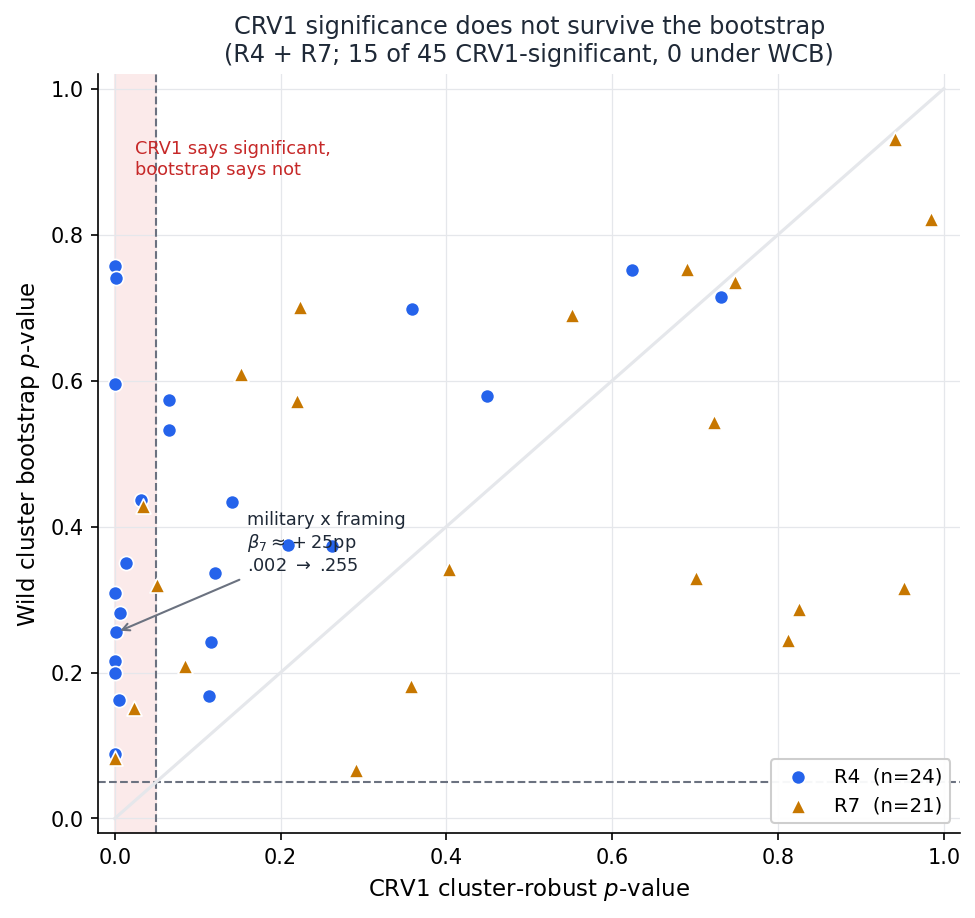
\includegraphics[width=0.72\linewidth]{figures/r4r7_crv1_vs_wcb.png}
  \caption{The CRV1-to-bootstrap collapse across both causal designs. Each point
  is one difference-in-differences estimate from R4 (per-event $\beta_3$ and
  crisis-type $\beta_7$) or R7 (per-event and pooled $\beta_3$); axes are its
  cluster-robust (CRV1) and wild-cluster-bootstrap $p$-values. Of 45 estimates,
  15 are CRV1-significant and \emph{none} survive the bootstrap: every point in
  the shaded CRV1-significant column sits above the $0.05$ line, and no point
  falls below the diagonal. The headline candidate --- military crises moving
  stake-holding communities toward security-and-military framing by
  $\beta_7\approx+25$pp --- moves from $p=0.002$ to $0.255$.}
  \label{fig:crv1-wcb}
\end{figure}

% =========================================================================
% OLD BULLET SPECIFICATION (commented out per Mohit: comment old, add new).
% Superseded by the prose above. Kept for traceability of the source numbers.
% Note: old spec said "R7: 0 of 7 cells" for the MDE; the analysis log gives
% 0 of 21 (ratios 0.04-0.47), corrected in the prose.
% =========================================================================
% \begin{description}
% \item[Setup.] Two independent causal designs: R4 (community-intensity DiD + crisis-type DDD)
%   and R7 (minority x acute DiD with subreddit and author FE).
% \item[R4 result.] CRV1 flags 9/18 per-event beta3 and 3/6 DDD beta7; WCB erases all
%   (0/18, 0/6, 0/8 on continuous Perspective toxicity). beta7 ~ +25pp moves p=0.002 -> WCB 0.255.
% \item[R7 result.] Pooled beta3 on log length -0.029 (CRV1 p=0.403, WCB p=0.342);
%   neutral sentiment p=0.023 -> WCB 0.151; 0 of 18 per-event survive.
% \item[The stronger point.] Parallel trends fail (R4: only Article 370 passes;
%   R7: all three, Wald chi2 48.8/31.3/21.7). Uninformative, not underpowered.
% \item[Why, structurally.] Crises cluster in time; each military pre-period is the
%   prior crisis aftermath. Structural confounder for crisis-response DiD.
% \item[Power.] R4 median MDE ~18pp, 0/18 detectable. R7: 0 of 7 [corrected: 0 of 21],
%   |beta3|/MDE 0.09-0.35 [corrected: 0.04-0.47].
% \item[Additional honesty.] WCB near validity floor at 7-9 clusters; over-conservative.
% \item[Descriptive residue.] R7: minority acute-phase commenters terser but less neutral.
% \item[Figures.] r7\_eventstudy\_logwords.png, r7\_mde.png, r4\_binned\_es\_secmil.png,
%   r4\_mde.png; Figure 8 = CRV1 vs WCB p-value scatter over 42 estimates.
% \item[Status.] Negative / methodological.
% \end{description}

%% ===========================================================================
\section{Discussion}
\budget{1,300}

\subsection{Composition is the unit of analysis}
\budget{250}

\jun{Prose draft (my part; old bullet spec commented below). Covers the R8-vs-R2
reconciliation the spec flagged.}

The findings converge on a single methodological point: none of them is visible
in one annotation layer. The affective-privileging result needs sentiment,
frame, stance, and community together; the boundary-crossing result needs a
thirteen-dimensional author fingerprint; and the contestation result \emph{is},
in effect, the failure of the single-layer account, since the offensiveness layer
that a content score would read barely moves the outcome. The object that carries
the signal is the composition of layers with community context, not any layer on
its own.

This raises an apparent tension worth resolving directly, because a reader will
otherwise find it. Our contestation result says toxicity scarcely drives what a
community argues over, while the reply-tree analysis says frame-crossing
\emph{carries} more toxicity. Both hold, and they are not in conflict: toxicity
travels \emph{with} the act of crossing a frame boundary without \emph{driving}
whether a community contests a comment. The variable that predicts contestation
is the frame--community pairing; toxicity is a correlate of one particular move
within the discourse, not the quantity that decides its reception.

We state the scope of the claim carefully. This is a demonstration on one corpus
and one conflict that compositional structure recovers what a single layer hides;
it is not a proof that composition always dominates, and the mechanism behind each
composition remains to be tested on other conflicts and platforms.

% OLD SPEC (superseded by prose above):
% \begin{itemize}
% \item No headline finding is visible in one layer. R5 needs L2xL5xL4xcommunity;
%   R6 needs a 13-dim fingerprint; R8's result IS the single-layer failure.
% \item Reconcile: R8 says toxicity barely moves contestation; R2 says
%   frame-crossing carries toxicity. Both hold: toxicity travels WITH crossing
%   but does not DRIVE contestation.
% \item Generalization: one corpus, one conflict; not a proof composition always beats layer.
% \end{itemize}

\subsection{Humanitarian framing as the permeable seam}
\budget{250}

\jun{Prose draft (my part; old bullet spec commented below). Corrected the
audience-heterogeneity point: we tested it (§5.6) rather than leaving it
unresolved, and updated the comments-per-author figures to the verified values.}

Humanitarian framing is the seam along which these communities come apart. It is
the one frame that both diverges affectively across communities and, in the
contestation analysis, cracks consensus within them: it is simultaneously the
most contested category overall and the most likely to split an aligned community
that would close ranks around a security-and-military frame. Offered as a
mechanism and not a tested claim, the reading is that security-and-military
framing invites a rally-round-the-flag response an aligned community can answer in
unison, whereas humanitarian framing forces a moral judgment that co-partisans
answer differently --- so the disagreement surfaces inside the community rather
than only across the line.

The obvious competing explanation is that general-audience communities look more
contested simply because they draw a more transient crowd, whose one-off voters
mechanically split the vote --- an audience-heterogeneity effect rather than a
permeable echo chamber. Neutral communities do have the most transient audience
(2.69 comments per author, against 4.50 in india-aligned and 5.04 in
pakistan-aligned communities), so we tested the explanation rather than assert
against it. It does not survive: controlling for author activity leaves the
neutral effect essentially unchanged, and restricting to committed participants
\emph{widens} rather than shrinks the gap (\S5.6). What the data cannot rule out
is a subtler, voter-level version --- heterogeneity among the people who cast
votes, which the corpus does not observe --- and we mark that as the open
condition rather than claim to have closed it.

% OLD SPEC (superseded by prose above):
% \begin{itemize}
% \item The one frame that both diverges affectively (S5.1, S5.3) and cracks
%   consensus within communities (S5.6).
% \item Mechanism (not test): Sec/Mil = rally-round-the-flag; Humanitarian =
%   moral judgment co-partisans answer differently.
% \item Competing explanation "data cannot rule out" -> CORRECTED: tested in S5.6
%   and rejected (author transience); only voter-pool version remains open.
%   Numbers 2.73/4.64/5.21 -> 2.69/4.50/5.04.
% \end{itemize}

\subsection{``Bridge user'' is the wrong abstraction}
\budget{220}

\begin{itemize}
\item The clustering failure and the raiding signature together argue that
  crossing is a behaviour with a distribution, not a user type, and that its
  modal form is antagonistic.
\item Any system that treats cross-community participation as a proxy for
  constructive participation will systematically boost incursions.
\item Extends Garimella et al.~\cite{garimella2018echo} beyond network position;
  instantiates Kumar et al.~\cite{kumar2018conflict} at the individual level;
  sits against Xia et al.~\cite{xia2025integrated}, who find at best conditional
  depolarization from cross-party contact.
\end{itemize}

\subsection{Measurement as a first-class finding}
\budget{150}

\dnote{New in v2.}

\begin{itemize}
\item The specification curve's largest variance source is \textbf{the
  labeller}, not any sampling or modelling choice.
\item Perspective --- the classifier platforms actually deploy --- is the
  \textbf{weakest instrument measured} ($\kappa$ 0.228--0.249) against a human
  ceiling of 0.682 on the same construct, and was run English-only on a 3.1\%
  code-mixed corpus.
\item No automated labeller reached the human ceiling on any layer, and that
  ceiling is itself only 0.45--0.68.
\item Consequence for CSCW practice: LLM-annotated corpora need a
  \textbf{labeller-comparison arm}, not a single validation number --- and
  reliability reporting has to acknowledge that the human ruler is noisy too.
\end{itemize}

\subsection{Design implications}
\budget{280}

Four, each traced to a specific finding, each with its own failure mode named.

\begin{description}
\item[Composition-aware moderation triage.] Surface high-harm cells
  (Humanitarian $\rightarrow$ Security/Military transitions; Religious/Cultural
  $\times$ Offensive-Targeted in acute phases) rather than ranking by toxicity
  score. \emph{Failure mode:} composition cells are community-specific and will
  not transfer across conflicts without re-estimation.

\item[Narrative-transparency affordance.] Show per-community frame--affect
  composition on a thread. \emph{Failure mode:} making affective asymmetry
  legible may harden identity rather than soften it
  (cf.~\cite{bail2018exposure}).

\item[Crossing-aware visibility floors.] A minimum-visibility guarantee for
  out-group comments, since the penalty falls on inquisitive and balanced voices
  alike (question\_rate OR 2.15). \emph{Failure mode:} the same floor protects
  provocateurs, who are most of the crossers.

\item[Crisis-phase-adaptive policy.] Moderation thresholds as a function of
  \texttt{crisis\_phase} $\times$ \texttt{crisis\_type}, justified by \S5.1's
  finding that crisis type --- not era --- determines the discourse regime.
  \emph{Failure mode:} \S5.7 shows the corpus cannot causally identify phase
  effects, so this is a hypothesis for a platform-side experiment, not a
  validated recommendation.
\end{description}

\subsection{Few clusters and the limits of crisis-response causal inference}
\budget{150}

\jun{Prose draft (my part, C3; old bullet spec commented below).}

The methodological negative generalizes beyond this corpus. Any crisis-response
study whose treatment varies across roughly six events and ten communities sits
in the same few-clusters regime, where the cluster-robust variance estimator
over-rejects and the wild cluster bootstrap is only barely valid --- so an
uncorrected event-study on data of this shape will report effects that a proper
correction erases, as ours did on both designs (\S5.7, Figure~\ref{fig:crv1-wcb}).
The compounding problem is identification rather than power: when crises recur
inside each other's recovery windows, each event's pre-period is the aftermath of
the last, and parallel trends fail structurally. There are two ways out --- redesign
toward many clusters (thread-level opinion climates, author panels) or frame the
account as descriptive --- and this paper takes the second and says so plainly.

% OLD SPEC (superseded by prose above):
% \begin{itemize}
% \item Generalize C3: ~6 events x 10 communities is the regime where CRV1 lies
%   and WCB is barely valid.
% \item Two routes out: many-cluster redesigns or explicit descriptive framing.
%   This paper takes the second.
% \end{itemize}


%% ===========================================================================
\section{Limitations}
\label{sec:limitations}
\budget{550}

\jun{Prose draft of the limitations, gathered here per the Sept.\ meeting
(all limitations in one dedicated section rather than scattered through Findings).
Content unchanged from the bullet list, which is commented out below; I prose-ified
the measurement, inference, and R7/R8 items and kept every fact. The Findings
mentions of these caveats are now compressed to a clause plus a pointer here.}

Several limitations bound these results, in roughly descending order of how much
they constrain the claims. The most pervasive is measurement. No annotation layer
reaches a Krippendorff $\alpha$ of 0.800, and only offensiveness-target (L6b, at
0.682) clears 0.667; the four-class content-type layer (L1) is too unreliable to
carry claims (machine $\kappa$ 0.368, a Factual-Claim recall of 4.8\%). Every
finding inherits this measurement error, and \S3.9 states the budget recipe by
recipe. Reliability is worst on the diaspora communities ($\kappa$ 0.273 for L1
and 0.404 for L5), which is one reason the diaspora ($N = 2{,}280$) is reported as
exploratory, in a single sentence with no modelled results.

Two structural features of the design limit what community comparisons can mean.
\texttt{community\_alignment} is a property of the venue read as a property of the
person: \S5.2's own within-alignment test shows the spread inside the
India-aligned communities (0.160) exceeds the gap across alignments (0.088), and
R1, R2, R5, and R8 all make this move while only R6 handles it at the author
level. Alignment is also perfectly collinear with subreddit --- ``general
audience'' is r/worldnews, r/geopolitics and r/lesscredibledefence together, and
the Pakistan-aligned group is the single community r/pakistan, so every
Pakistan-aligned claim is really a claim about that one community.

The outcome measures carry their own caveats, which matter most for the
contestation result (R8). Three of the headline findings ride the same platform
vote signal --- \texttt{score\_log}, a median split of \texttt{score}, and
\texttt{controversiality} --- so they are less independent than they look. And
\texttt{controversiality} itself conflates contested with merely downvoted:
23.8\% of comments at a net score of zero or below are flagged against 0.02\% of
those above one hundred, and the flag is platform metadata rather than observed
deliberation, which is why we speak of contested \emph{reception} throughout
rather than debate. Collection is also asymmetric: Operation Sindoor is 43\% of
the crisis corpus and twelve times the size of Pulwama, so genuine engagement
growth cannot be cleanly separated from retrieval completeness; our robustness is
by exclusion rather than correction, and R8 does not yet carry that exclusion arm.
Thread depth is lost non-randomly with respect to frame (15.8\% of comments
unresolved, 73.9\% for Historical Grievance against 87.3\% for
Security/Military), and Historical Grievance also carries the largest
depth-growth claim.

The causal analyses (R4, R7) are the sharpest limitation, and \S5.7 documents it
in full: no causal identification survives the wild cluster bootstrap, so the
paper is associational throughout. Two design-specific caveats attach to R7. Its
lean rule discards 50.6\% of aligned-community comments and treats anti-Pakistan
as pro-India without separate validation. And both of R7's silencing channels
inherit limits the design cannot beat: the expression channel is a null, while the
participation channel (comment counts) shows a spiral-direction descriptive signal
that does not survive the bootstrap and rests on a survivorship-limited panel,
since authors already silent in the baseline are unobservable.

Finally, two scope limits. Roughly 3.1\% of the corpus is code-mixed Hindi/Urdu or
transliterated, but the gold samples contain only 8, 8, and 13 such items, so a
separate $\kappa$ cannot be estimated and the Perspective scores were computed
English-only. And the qualitative arm is single-analyst until the two-coder pass
is complete, which is why \S4.4 describes it as analyst close reading.

% =========================================================================
% OLD BULLET SPECIFICATION (commented out; prose above gathers all limitations
% here per the Sept. meeting. Every fact preserved.)
% =========================================================================
% \begin{enumerate}
% \item No layer reaches Krippendorff alpha >= 0.800; only L6b (0.682) clears 0.667.
%   L1 unusable (kappa 0.368, Factual Claim recall 4.8%). S3.9 budget per recipe.
% \item Associational throughout; no causal identification survives; S5.7 why.
% \item community_alignment is venue read as person (V3). S5.2 within-alignment
%   spread 0.160 > across-alignment 0.088. R1,R2,R5,R8 do this; only R6 handles it.
% \item Alignment collinear with subreddit (V7). Neutral = worldnews+geopolitics+
%   lesscredibledefence; pakistan_aligned = single subreddit r/pakistan.
% \item Three headline findings ride the same vote signal (score_log, score,
%   controversiality) (V2).
% \item controversiality conflates contested with downvoted (23.8% at score<=0 vs
%   0.02% at 100+); platform metadata, not deliberation.
% \item Collection asymmetry: Sindoor 43% of crisis corpus, 12x Pulwama;
%   robustness by exclusion; R8 has no exclusion arm (B9).
% \item Depth loss systematic on frame (15.8% unresolved; HG 73.9% vs SM 87.3%).
% \item Language coverage: 3.1% code-mixed; gold has only 8/8/13; Perspective English-only.
% \item Qualitative arm single-analyst until two-coder pass (B8); S4.4 says so.
% \item R7 lean rule discards 50.6% of aligned comments; conflates anti-Pak with pro-India.
% \item Diaspora (N=2,280) exploratory only; reliability worst (L1 0.273, L5 0.404).
% \end{enumerate}


%% ===========================================================================
\section{Conclusion}
\budget{250}

\begin{itemize}
\item Restate the thesis with the two numbers that do the most work: neutral
  $\times$ Humanitarian \textbf{17.4\%} against the Offensive-versus-not gap of
  \textbf{7.67\% / 6.83\%}; and the Security/Military positivity asymmetry
  (0.094 india versus 0.050 neutral).
\item One sentence on what the negative results buy --- the event-clustering
  confounder, the continuum finding, and the labeller comparison are all results
  the paper only has because it reported failures.
\item \textbf{No future-work laundry list.} One concrete next step: the L7
  veracity layer over the gated Factual Claims, which requires first fixing an L1
  gate that currently recovers 4.8\% of them.
\end{itemize}


%% ===========================================================================
%% BACK MATTER
%% ===========================================================================

\section*{Required statements}
\addcontentsline{toc}{section}{Required statements}

Data Availability; Ethics Declaration; Author Contributions (CRediT); Conflict
of Interest; Funding; \textbf{AI-Use Statement}.

% \begin{acks}
%   Placeholder. Identification of funding sources and other support, and thanks
%   to individuals and groups that assisted in the research and the preparation of
%   the work, go here. Remove for double-anonymous review.
% \end{acks}


\bibliographystyle{ACM-Reference-Format}
\bibliography{paper_cscw}

%% ===========================================================================
\appendix


%% ===========================================================================
\section{R8 large-N robustness: effect sizes and equivalence tests}
\label{app:r8equiv}

% tab_r8equiv.tex -- R8 large-N robustness (effect sizes + within-frame equivalence)
\begin{table}[H]
\centering
\caption{Large-sample robustness for the contestation result. Top: N-independent
effect sizes (Cramer's V) for the three factors, with the descriptive max/min
rate ratio for reference; all three associations are small in absolute terms and
their rank is community $>$ frame $>$ offensiveness. Bottom: the within-frame
offensive-versus-not contrast, with 95\% CI, effect size $\phi$, and a TOST
equivalence test against a $\pm 2$pp margin. Numbers from
\texttt{scripts/r8\_toxicity\_equivalence.py}.}
\label{tab:r8equiv}
\setlength{\tabcolsep}{5pt}
\footnotesize
\begin{tabularx}{\linewidth}{@{}>{\raggedright\arraybackslash}Xrrr@{}}
\toprule
\multicolumn{4}{@{}l}{\emph{Effect sizes (contestation $\sim$ factor)}} \\
factor & rate ratio & Cramer's $V$ & interpretation \\
\midrule
community    & 2.47$\times$ & 0.114 & weak \\
frame        & 1.77$\times$ & 0.040 & negligible \\
offensiveness & 1.12$\times$ & 0.009 & negligible \\
\bottomrule
\end{tabularx}

\vspace{4pt}

\begin{tabularx}{\linewidth}{@{}>{\raggedright\arraybackslash}Xrrrr@{}}
\toprule
\multicolumn{5}{@{}l}{\emph{Within-frame offensive vs.\ not ($\Delta$ = offensive $-$ not)}} \\
frame & $\Delta$ (pp) & 95\% CI (pp) & $\phi$ & TOST \\
\midrule
Humanitarian         & $-0.29$ & $[-1.80, +1.21]$ & 0.003 & equiv. \\
Historical Grievance & $+0.74$ & $[-1.02, +2.50]$ & 0.007 & n.s.\ \\
Political            & $+1.00$ & $[+0.51, +1.49]$ & 0.012 & equiv. \\
Religious/Cultural   & $-0.52$ & $[-1.47, +0.43]$ & 0.007 & equiv. \\
Security/Military    & $+0.60$ & $[+0.10, +1.11]$ & 0.007 & equiv. \\
Economic             & $+1.85$ & $[+0.01, +3.69]$ & 0.019 & n.s.\ \\
\bottomrule
\end{tabularx}

\vspace{2pt}
{\footnotesize ``equiv.'' marks a frame where the $\pm 2$pp equivalence test
rejects at $p < 0.05$. The two ``n.s.'' frames are under-powered for equivalence
(small offensive $n$ widens the CI), not evidence of a large gap: both have
$\phi < 0.02$.}
\end{table}



%% ===========================================================================
\section{Figure plan}


%% Example figure stub -- uncomment and point at a real file once figures are
%% copied into the Overleaf project.
%%
%% \begin{figure}[h]
%%   \centering
%%   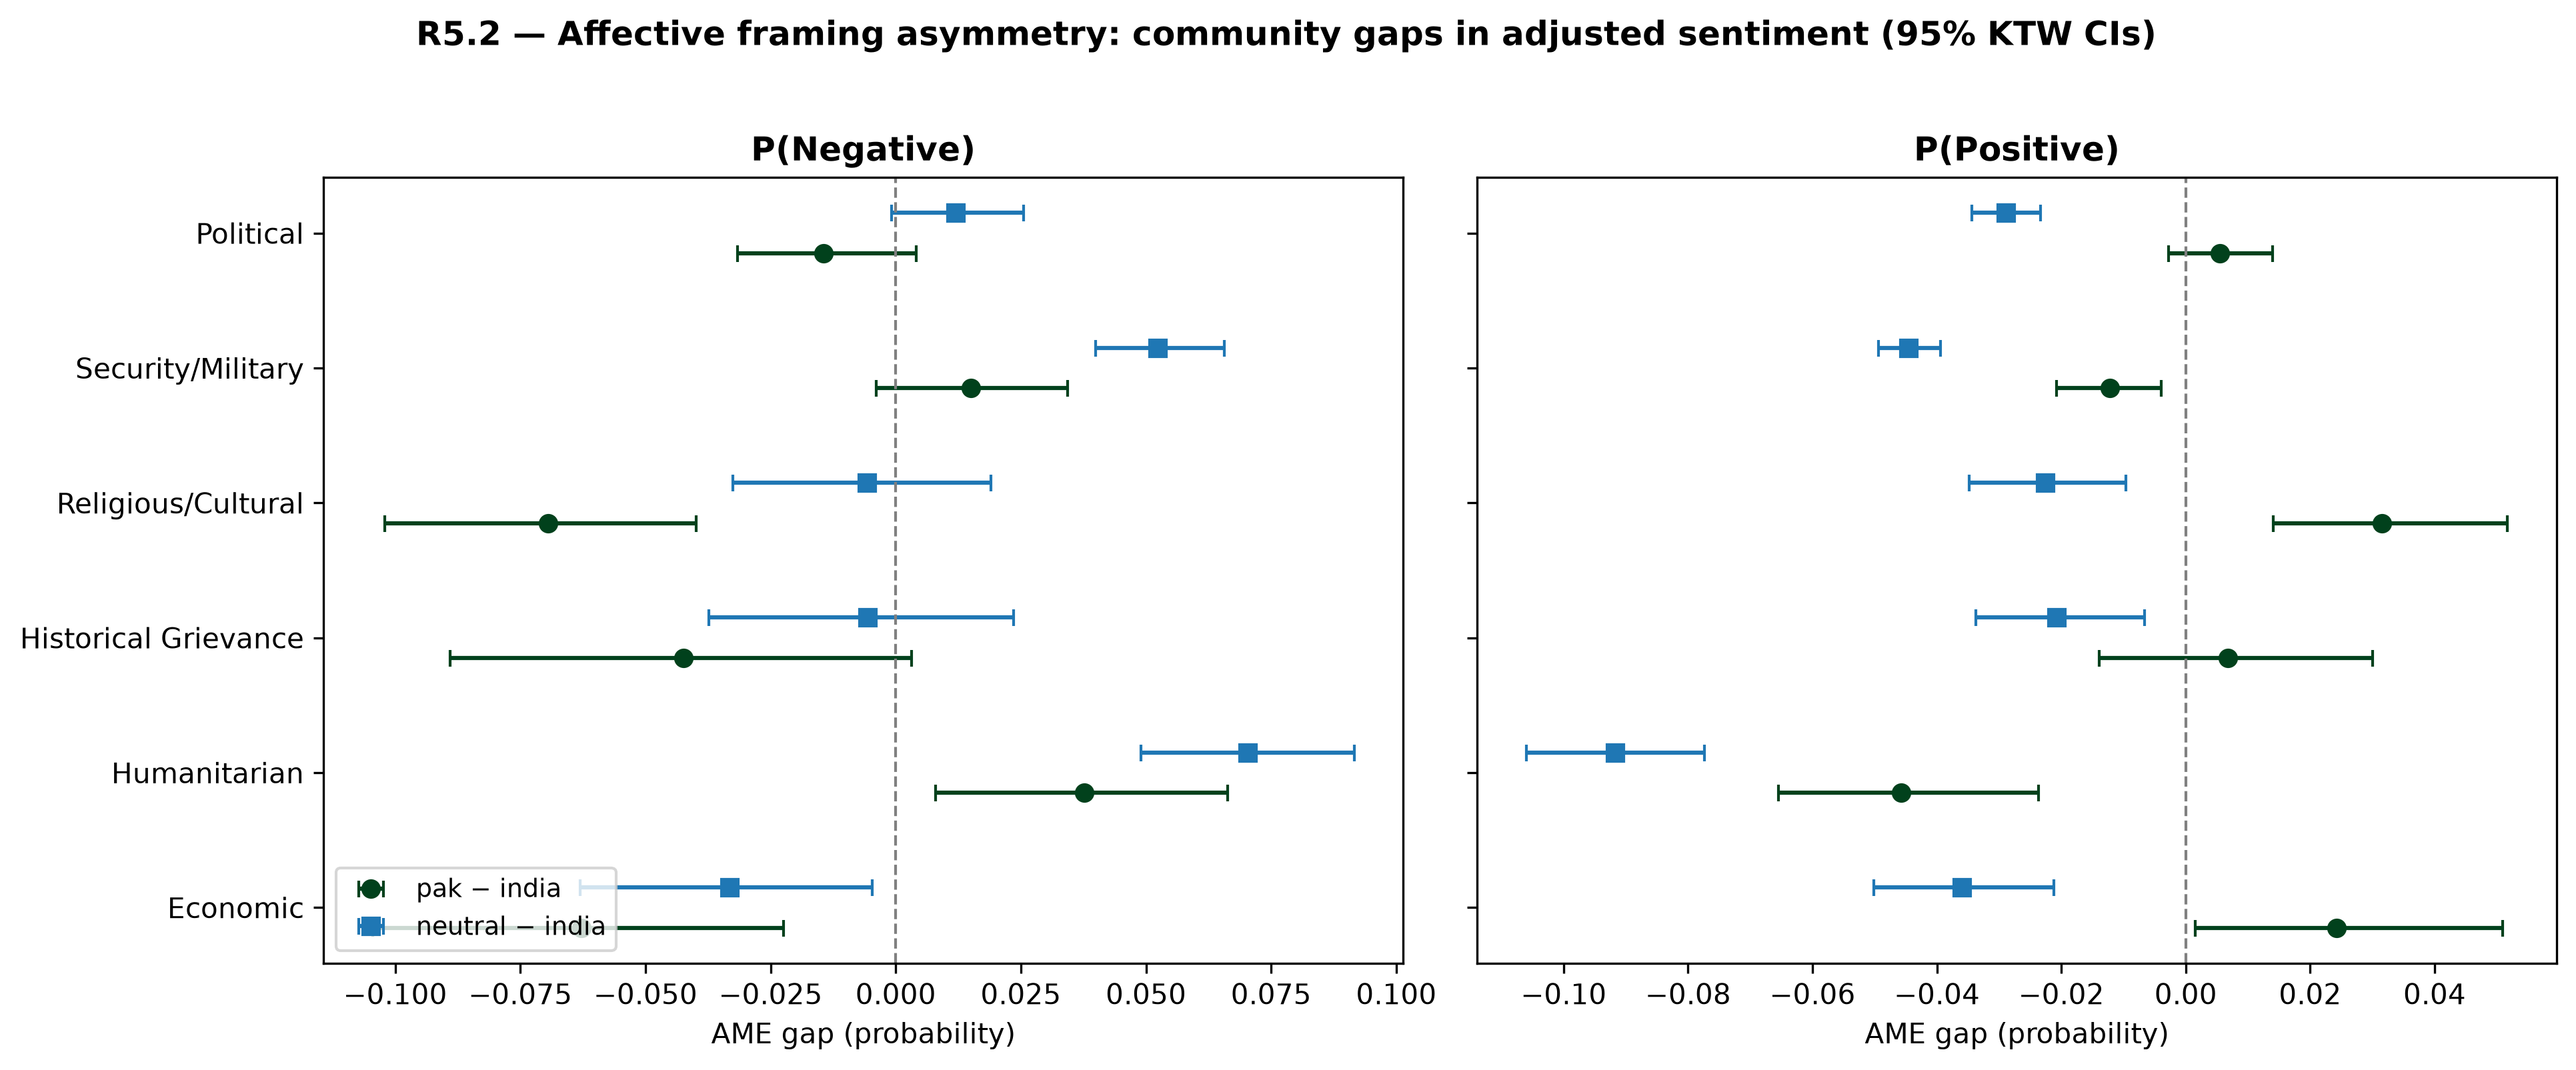
\includegraphics[width=\linewidth]{r5_ame_plot}
%%   \caption{Average marginal effects on P(Negative) and P(Positive) by frame
%%     and community, with King-Tomz-Wittenberg simulation CIs.}
%%   \Description{TODO: plain-text description under 2000 characters.}
%%   \label{fig:ame}
%% \end{figure}


\end{document}
